%% Reporte técnico — Predicción multiclase de deserción estudiantil con métodos de ensamble
%% Plantilla IEEE Conference (IEEEtran). Compilar: pdflatex main && bibtex main && pdflatex main && pdflatex main
%% Las cifras del texto provienen de tables/numbers.tex y de tables/*.tex, generados por scripts/make_tables.py
\documentclass[conference]{IEEEtran}

\usepackage[utf8]{inputenc}
\usepackage[T1]{fontenc}
\usepackage[spanish,es-tabla,es-nodecimaldot]{babel}
\usepackage{amsmath,amssymb}
\usepackage{graphicx}
\usepackage{booktabs}
\usepackage{array}
\usepackage{xcolor}
\usepackage{tikz}
\usetikzlibrary{babel,arrows.meta,positioning,calc}
\usepackage{cite}
\usepackage{url}
\usepackage{balance}
\usepackage{microtype}
\usepackage[hidelinks]{hyperref}

% --- Datos del autor y del repositorio (editar aquí) ------------------------------------------------------------
\newcommand{\correo}{\texttt{TU\_CORREO@uach.mx}}                      % <-- PENDIENTE: poner el correo real
\newcommand{\repoURL}{https://github.com/JonahGGC/proyecto-final-ml}   % <-- PENDIENTE: confirmar la URL del repositorio

% --- Cifras generadas por scripts/make_tables.py -----------------------------------------------------------------
% Generado por scripts/make_tables.py — no editar a mano
\newcommand{\Nte}{885}
\newcommand{\Ntot}{4,424}
\newcommand{\Ntr}{3,539}
\newcommand{\accLRD}{0.771}
\newcommand{\auMax}{+0.006}
\newcommand{\auMin}{$-$0.010}
\newcommand{\cursoMax}{55.7}
\newcommand{\cursoMin}{14.8}
\newcommand{\cursoSinUC}{171}
\newcommand{\cvAccADA}{0.756}
\newcommand{\cvAccADAB}{0.727}
\newcommand{\cvAccBAG}{0.760}
\newcommand{\cvAccBAGB}{0.747}
\newcommand{\cvAccDT}{0.692}
\newcommand{\cvAccDUM}{0.499}
\newcommand{\cvAccEBM}{0.768}
\newcommand{\cvAccEBMB}{0.766}
\newcommand{\cvAccEBMG}{0.752}
\newcommand{\cvAccGB}{0.773}
\newcommand{\cvAccGBB}{0.771}
\newcommand{\cvAccHGB}{0.778}
\newcommand{\cvAccHGBB}{0.770}
\newcommand{\cvAccLR}{0.758}
\newcommand{\cvAccLRD}{0.776}
\newcommand{\cvAccPAS}{0.764}
\newcommand{\cvAccPASB}{0.743}
\newcommand{\cvAccRF}{0.769}
\newcommand{\cvAccRFB}{0.766}
\newcommand{\cvAccSTK}{0.775}
\newcommand{\cvAccSTKB}{0.759}
\newcommand{\cvAccSVL}{0.772}
\newcommand{\cvAccSVLD}{0.772}
\newcommand{\cvAccSVP}{0.761}
\newcommand{\cvAccSVPD}{0.752}
\newcommand{\cvAccSVR}{0.787}
\newcommand{\cvAccSVRD}{0.772}
\newcommand{\cvAccVH}{0.779}
\newcommand{\cvAccVHB}{0.780}
\newcommand{\cvAccVS}{0.786}
\newcommand{\cvAccVSB}{0.790}
\newcommand{\cvFADA}{0.718}
\newcommand{\cvFADAB}{0.678}
\newcommand{\cvFBAG}{0.710}
\newcommand{\cvFBAGB}{0.702}
\newcommand{\cvFDT}{0.656}
\newcommand{\cvFDUM}{0.222}
\newcommand{\cvFEBM}{0.731}
\newcommand{\cvFEBMB}{0.728}
\newcommand{\cvFEBMG}{0.714}
\newcommand{\cvFGB}{0.732}
\newcommand{\cvFGBB}{0.730}
\newcommand{\cvFHGB}{0.734}
\newcommand{\cvFHGBB}{0.716}
\newcommand{\cvFLR}{0.717}
\newcommand{\cvFLRD}{0.701}
\newcommand{\cvFMaxOpt}{0.737}
\newcommand{\cvFMinOpt}{0.710}
\newcommand{\cvFPAS}{0.719}
\newcommand{\cvFPASB}{0.700}
\newcommand{\cvFRF}{0.726}
\newcommand{\cvFRFB}{0.718}
\newcommand{\cvFSTK}{0.733}
\newcommand{\cvFSTKB}{0.722}
\newcommand{\cvFSVL}{0.709}
\newcommand{\cvFSVLD}{0.681}
\newcommand{\cvFSVP}{0.721}
\newcommand{\cvFSVPD}{0.664}
\newcommand{\cvFSVR}{0.722}
\newcommand{\cvFSVRD}{0.691}
\newcommand{\cvFVH}{0.737}
\newcommand{\cvFVHB}{0.729}
\newcommand{\cvFVS}{0.737}
\newcommand{\cvFVSB}{0.726}
\newcommand{\cvFqADA}{0.718}
\newcommand{\cvFqADAB}{0.678}
\newcommand{\cvFqBAG}{0.710}
\newcommand{\cvFqBAGB}{0.702}
\newcommand{\cvFqDT}{0.656}
\newcommand{\cvFqDUM}{0.222}
\newcommand{\cvFqEBM}{0.731}
\newcommand{\cvFqEBMB}{0.728}
\newcommand{\cvFqEBMG}{0.714}
\newcommand{\cvFqGB}{0.732}
\newcommand{\cvFqGBB}{0.730}
\newcommand{\cvFqHGB}{0.734}
\newcommand{\cvFqHGBB}{0.716}
\newcommand{\cvFqLR}{0.717}
\newcommand{\cvFqLRD}{0.701}
\newcommand{\cvFqLRR}{0.715}
\newcommand{\cvFqPAS}{0.719}
\newcommand{\cvFqPASB}{0.700}
\newcommand{\cvFqRF}{0.726}
\newcommand{\cvFqRFB}{0.718}
\newcommand{\cvFqSTK}{0.733}
\newcommand{\cvFqSTKB}{0.722}
\newcommand{\cvFqSVL}{0.709}
\newcommand{\cvFqSVLD}{0.681}
\newcommand{\cvFqSVP}{0.721}
\newcommand{\cvFqSVPD}{0.664}
\newcommand{\cvFqSVR}{0.722}
\newcommand{\cvFqSVRD}{0.691}
\newcommand{\cvFqVH}{0.737}
\newcommand{\cvFqVHB}{0.729}
\newcommand{\cvFqVS}{0.737}
\newcommand{\cvFqVSB}{0.726}
\newcommand{\cvGapADA}{0.087}
\newcommand{\cvGapADAB}{0.006}
\newcommand{\cvGapBAG}{0.171}
\newcommand{\cvGapBAGB}{0.052}
\newcommand{\cvGapDT}{0.087}
\newcommand{\cvGapDUM}{0.000}
\newcommand{\cvGapEBM}{0.064}
\newcommand{\cvGapEBMB}{0.057}
\newcommand{\cvGapEBMG}{0.043}
\newcommand{\cvGapGB}{0.185}
\newcommand{\cvGapGBB}{0.167}
\newcommand{\cvGapHGB}{0.213}
\newcommand{\cvGapHGBB}{0.282}
\newcommand{\cvGapLR}{0.033}
\newcommand{\cvGapLRD}{0.039}
\newcommand{\cvGapPAS}{0.193}
\newcommand{\cvGapPASB}{0.065}
\newcommand{\cvGapRF}{0.203}
\newcommand{\cvGapRFB}{0.146}
\newcommand{\cvGapSTK}{0.148}
\newcommand{\cvGapSTKB}{0.083}
\newcommand{\cvGapSVL}{0.024}
\newcommand{\cvGapSVLD}{0.038}
\newcommand{\cvGapSVP}{0.103}
\newcommand{\cvGapSVPD}{0.137}
\newcommand{\cvGapSVR}{0.043}
\newcommand{\cvGapSVRD}{0.103}
\newcommand{\cvGapVH}{0.191}
\newcommand{\cvGapVHB}{0.077}
\newcommand{\cvGapVS}{0.178}
\newcommand{\cvGapVSB}{0.052}
\newcommand{\cvMccADA}{0.614}
\newcommand{\cvMccADAB}{0.562}
\newcommand{\cvMccBAG}{0.610}
\newcommand{\cvMccBAGB}{0.596}
\newcommand{\cvMccDT}{0.525}
\newcommand{\cvMccDUM}{0.000}
\newcommand{\cvMccEBM}{0.634}
\newcommand{\cvMccEBMB}{0.631}
\newcommand{\cvMccEBMG}{0.610}
\newcommand{\cvMccGB}{0.636}
\newcommand{\cvMccGBB}{0.634}
\newcommand{\cvMccHGB}{0.642}
\newcommand{\cvMccHGBB}{0.624}
\newcommand{\cvMccLR}{0.618}
\newcommand{\cvMccLRD}{0.629}
\newcommand{\cvMccPAS}{0.619}
\newcommand{\cvMccPASB}{0.593}
\newcommand{\cvMccRF}{0.627}
\newcommand{\cvMccRFB}{0.620}
\newcommand{\cvMccSTK}{0.641}
\newcommand{\cvMccSTKB}{0.623}
\newcommand{\cvMccSVL}{0.623}
\newcommand{\cvMccSVLD}{0.623}
\newcommand{\cvMccSVP}{0.622}
\newcommand{\cvMccSVPD}{0.590}
\newcommand{\cvMccSVR}{0.648}
\newcommand{\cvMccSVRD}{0.623}
\newcommand{\cvMccVH}{0.644}
\newcommand{\cvMccVHB}{0.640}
\newcommand{\cvMccVS}{0.651}
\newcommand{\cvMccVSB}{0.652}
\newcommand{\cvSADA}{0.019}
\newcommand{\cvSADAB}{0.013}
\newcommand{\cvSBAG}{0.019}
\newcommand{\cvSBAGB}{0.013}
\newcommand{\cvSDT}{0.020}
\newcommand{\cvSDUM}{0.000}
\newcommand{\cvSEBM}{0.014}
\newcommand{\cvSEBMB}{0.009}
\newcommand{\cvSEBMG}{0.018}
\newcommand{\cvSGB}{0.019}
\newcommand{\cvSGBB}{0.021}
\newcommand{\cvSHGB}{0.019}
\newcommand{\cvSHGBB}{0.016}
\newcommand{\cvSLR}{0.019}
\newcommand{\cvSLRD}{0.019}
\newcommand{\cvSPAS}{0.020}
\newcommand{\cvSPASB}{0.016}
\newcommand{\cvSRF}{0.022}
\newcommand{\cvSRFB}{0.022}
\newcommand{\cvSSTK}{0.018}
\newcommand{\cvSSTKB}{0.021}
\newcommand{\cvSSVL}{0.019}
\newcommand{\cvSSVLD}{0.017}
\newcommand{\cvSSVP}{0.011}
\newcommand{\cvSSVPD}{0.020}
\newcommand{\cvSSVR}{0.011}
\newcommand{\cvSSVRD}{0.025}
\newcommand{\cvSVH}{0.019}
\newcommand{\cvSVHB}{0.018}
\newcommand{\cvSVS}{0.022}
\newcommand{\cvSVSB}{0.018}
\newcommand{\dcvADA}{+0.039}
\newcommand{\dcvBAG}{+0.008}
\newcommand{\dcvEBM}{+0.002}
\newcommand{\dcvGB}{+0.002}
\newcommand{\dcvHGB}{+0.018}
\newcommand{\dcvLR}{+0.016}
\newcommand{\dcvMax}{+0.039}
\newcommand{\dcvMedia}{+0.013}
\newcommand{\dcvMin}{+0.002}
\newcommand{\dcvPAS}{+0.018}
\newcommand{\dcvRF}{+0.009}
\newcommand{\dcvSTK}{+0.011}
\newcommand{\dcvSVL}{+0.028}
\newcommand{\dcvSVP}{+0.057}
\newcommand{\dcvSVR}{+0.031}
\newcommand{\dcvVH}{+0.008}
\newcommand{\dcvVS}{+0.012}
\newcommand{\detADA}{186}
\newcommand{\detBAG}{202}
\newcommand{\detEBM}{195}
\newcommand{\detGB}{198}
\newcommand{\detHGB}{197}
\newcommand{\detLR}{195}
\newcommand{\detLRR}{203}
\newcommand{\detPAS}{204}
\newcommand{\detRF}{201}
\newcommand{\detSTK}{199}
\newcommand{\detSVR}{208}
\newcommand{\detVH}{201}
\newcommand{\detVS}{203}
\newcommand{\dtcADA}{$-$0.040}
\newcommand{\dtcADAB}{$-$0.002}
\newcommand{\dtcBAG}{+0.003}
\newcommand{\dtcBAGB}{$-$0.018}
\newcommand{\dtcDT}{$-$0.030}
\newcommand{\dtcDUM}{+0.000}
\newcommand{\dtcEBM}{$-$0.034}
\newcommand{\dtcEBMB}{$-$0.034}
\newcommand{\dtcEBMG}{$-$0.023}
\newcommand{\dtcGB}{$-$0.044}
\newcommand{\dtcGBB}{$-$0.038}
\newcommand{\dtcHGB}{$-$0.059}
\newcommand{\dtcHGBB}{$-$0.033}
\newcommand{\dtcLR}{$-$0.029}
\newcommand{\dtcLRD}{$-$0.002}
\newcommand{\dtcLRR}{$-$0.031}
\newcommand{\dtcPAS}{$-$0.009}
\newcommand{\dtcPASB}{$-$0.020}
\newcommand{\dtcRF}{$-$0.010}
\newcommand{\dtcRFB}{$-$0.020}
\newcommand{\dtcSTK}{$-$0.036}
\newcommand{\dtcSTKB}{$-$0.020}
\newcommand{\dtcSVL}{$-$0.001}
\newcommand{\dtcSVLD}{$-$0.010}
\newcommand{\dtcSVP}{$-$0.025}
\newcommand{\dtcSVPD}{$-$0.032}
\newcommand{\dtcSVR}{$-$0.032}
\newcommand{\dtcSVRD}{+0.002}
\newcommand{\dtcVH}{$-$0.044}
\newcommand{\dtcVHB}{$-$0.030}
\newcommand{\dtcVS}{$-$0.035}
\newcommand{\dtcVSB}{$-$0.026}
\newcommand{\dteADA}{+0.001}
\newcommand{\dteBAG}{+0.029}
\newcommand{\dteEBM}{+0.002}
\newcommand{\dteGB}{$-$0.005}
\newcommand{\dteHGB}{$-$0.008}
\newcommand{\dteLR}{$-$0.011}
\newcommand{\dteMedia}{+0.006}
\newcommand{\dtePAS}{+0.029}
\newcommand{\dteRF}{+0.018}
\newcommand{\dteSTK}{$-$0.005}
\newcommand{\dteSVL}{+0.038}
\newcommand{\dteSVP}{+0.065}
\newcommand{\dteSVR}{$-$0.003}
\newcommand{\dteVH}{$-$0.006}
\newcommand{\dteVS}{+0.003}
\newcommand{\edadMax}{70}
\newcommand{\edadMin}{17}
\newcommand{\falsaADA}{37}
\newcommand{\falsaBAG}{45}
\newcommand{\falsaEBM}{43}
\newcommand{\falsaGB}{48}
\newcommand{\falsaHGB}{57}
\newcommand{\falsaLR}{42}
\newcommand{\falsaLRR}{50}
\newcommand{\falsaPAS}{46}
\newcommand{\falsaRF}{38}
\newcommand{\falsaSTK}{46}
\newcommand{\falsaSVR}{55}
\newcommand{\falsaVH}{49}
\newcommand{\falsaVS}{51}
\newcommand{\fuDADA}{0.734}
\newcommand{\fuDADAB}{0.734}
\newcommand{\fuDBAG}{0.761}
\newcommand{\fuDBAGB}{0.740}
\newcommand{\fuDDT}{0.685}
\newcommand{\fuDDUM}{0.000}
\newcommand{\fuDEBM}{0.747}
\newcommand{\fuDEBMB}{0.746}
\newcommand{\fuDEBMG}{0.748}
\newcommand{\fuDGB}{0.747}
\newcommand{\fuDGBB}{0.749}
\newcommand{\fuDHGB}{0.732}
\newcommand{\fuDHGBB}{0.751}
\newcommand{\fuDLR}{0.749}
\newcommand{\fuDLRD}{0.766}
\newcommand{\fuDLRR}{0.756}
\newcommand{\fuDPAS}{0.764}
\newcommand{\fuDPASB}{0.744}
\newcommand{\fuDRF}{0.769}
\newcommand{\fuDRFB}{0.749}
\newcommand{\fuDSTK}{0.752}
\newcommand{\fuDSTKB}{0.756}
\newcommand{\fuDSVL}{0.752}
\newcommand{\fuDSVLD}{0.762}
\newcommand{\fuDSVP}{0.746}
\newcommand{\fuDSVPD}{0.739}
\newcommand{\fuDSVR}{0.761}
\newcommand{\fuDSVRD}{0.773}
\newcommand{\fuDVH}{0.753}
\newcommand{\fuDVHB}{0.756}
\newcommand{\fuDVS}{0.755}
\newcommand{\fuDVSB}{0.766}
\newcommand{\fuEADA}{0.485}
\newcommand{\fuEADAB}{0.471}
\newcommand{\fuEBAG}{0.523}
\newcommand{\fuEBAGB}{0.490}
\newcommand{\fuEDT}{0.444}
\newcommand{\fuEDUM}{0.000}
\newcommand{\fuEEBM}{0.517}
\newcommand{\fuEEBMB}{0.512}
\newcommand{\fuEEBMG}{0.503}
\newcommand{\fuEGB}{0.482}
\newcommand{\fuEGBB}{0.497}
\newcommand{\fuEHGB}{0.460}
\newcommand{\fuEHGBB}{0.464}
\newcommand{\fuELR}{0.493}
\newcommand{\fuELRD}{0.468}
\newcommand{\fuELRR}{0.473}
\newcommand{\fuEPAS}{0.520}
\newcommand{\fuEPASB}{0.480}
\newcommand{\fuERF}{0.532}
\newcommand{\fuERFB}{0.497}
\newcommand{\fuESTK}{0.500}
\newcommand{\fuESTKB}{0.516}
\newcommand{\fuESVL}{0.505}
\newcommand{\fuESVLD}{0.397}
\newcommand{\fuESVP}{0.511}
\newcommand{\fuESVPD}{0.324}
\newcommand{\fuESVR}{0.451}
\newcommand{\fuESVRD}{0.447}
\newcommand{\fuEVH}{0.483}
\newcommand{\fuEVHB}{0.494}
\newcommand{\fuEVS}{0.499}
\newcommand{\fuEVSB}{0.474}
\newcommand{\fuGADA}{0.813}
\newcommand{\fuGADAB}{0.825}
\newcommand{\fuGBAG}{0.855}
\newcommand{\fuGBAGB}{0.822}
\newcommand{\fuGDT}{0.748}
\newcommand{\fuGDUM}{0.666}
\newcommand{\fuGEBM}{0.826}
\newcommand{\fuGEBMB}{0.826}
\newcommand{\fuGEBMG}{0.824}
\newcommand{\fuGGB}{0.832}
\newcommand{\fuGGBB}{0.831}
\newcommand{\fuGHGB}{0.834}
\newcommand{\fuGHGBB}{0.834}
\newcommand{\fuGLR}{0.824}
\newcommand{\fuGLRD}{0.863}
\newcommand{\fuGLRR}{0.821}
\newcommand{\fuGPAS}{0.845}
\newcommand{\fuGPASB}{0.817}
\newcommand{\fuGRF}{0.848}
\newcommand{\fuGRFB}{0.847}
\newcommand{\fuGSTK}{0.839}
\newcommand{\fuGSTKB}{0.834}
\newcommand{\fuGSVL}{0.866}
\newcommand{\fuGSVLD}{0.852}
\newcommand{\fuGSVP}{0.830}
\newcommand{\fuGSVPD}{0.831}
\newcommand{\fuGSVR}{0.858}
\newcommand{\fuGSVRD}{0.858}
\newcommand{\fuGVH}{0.843}
\newcommand{\fuGVHB}{0.847}
\newcommand{\fuGVS}{0.855}
\newcommand{\fuGVSB}{0.860}
\newcommand{\gAprobCero}{0.0}
\newcommand{\gSinUC}{43.2}
\newcommand{\impRFAPri}{0.027}
\newcommand{\impRFASeg}{0.072}
\newcommand{\impRFTF}{0.042}
\newcommand{\impVSAPri}{0.056}
\newcommand{\impVSASeg}{0.189}
\newcommand{\impVSTF}{0.045}
\newcommand{\mcnVS}{55 contra 28 ($p=0.004$)}
\newcommand{\nAprobCero}{557}
\newcommand{\nAprobCeroU}{434}
\newcommand{\nBin}{8}
\newcommand{\nCatOrig}{209}
\newcommand{\nCols}{106}
\newcommand{\nCompCV}{11}
\newcommand{\nCorrAlta}{4}
\newcommand{\nCursos}{17}
\newcommand{\nCursosGr}{15}
\newcommand{\nDB}{389}
\newcommand{\nEnsGen}{10}
\newcommand{\nHolmSig}{0}
\newcommand{\nMcnHolm}{4}
\newcommand{\nModGen}{12}
\newcommand{\nNF}{419}
\newcommand{\nNom}{9}
\newcommand{\nNum}{19}
\newcommand{\nOH}{79}
\newcommand{\nOptMejoraCV}{10}
\newcommand{\nOptMejoraTest}{6}
\newcommand{\nOutEdad}{358}
\newcommand{\nPareadas}{11}
\newcommand{\nParesNum}{171}
\newcommand{\nPcrudoSig}{2}
\newcommand{\nSinUC}{148}
\newcommand{\ntD}{1,421}
\newcommand{\ntE}{794}
\newcommand{\ntG}{2,209}
\newcommand{\nteD}{284}
\newcommand{\nteE}{159}
\newcommand{\nteG}{442}
\newcommand{\ntrD}{1,137}
\newcommand{\ntrE}{635}
\newcommand{\ntrG}{1,767}
\newcommand{\optMax}{0.009}
\newcommand{\optMaxAbs}{0.009}
\newcommand{\optMin}{$-$0.001}
\newcommand{\pCVTest}{0.37}
\newcommand{\pGap}{0.58}
\newcommand{\pOutEdad}{10.1}
\newcommand{\parBAG}{$+0.030$ ($[0.001,\,0.059]$)}
\newcommand{\parRF}{$+0.033$ (IC 95\,\% $[0.006,\,0.060]$)}
\newcommand{\parSVRAcc}{$+0.037$ ($[0.014,\,0.061]$)}
\newcommand{\parSVRAuc}{$-0.031$ ($[-0.044,\,-0.018]$)}
\newcommand{\parVSAcc}{$+0.031$ ($[0.010,\,0.051]$)}
\newcommand{\parVSF}{$+0.020$ ($[-0.005,\,0.043]$)}
\newcommand{\parVSMcc}{$+0.035$ ($[0.004,\,0.066]$)}
\newcommand{\perdidaMax}{0.059}
\newcommand{\perdidaMedia}{0.031}
\newcommand{\perdidaMin}{0.003}
\newcommand{\phoADA}{1.000}
\newcommand{\phoBAG}{0.043}
\newcommand{\phoEBM}{1.000}
\newcommand{\phoGB}{1.000}
\newcommand{\phoHGB}{1.000}
\newcommand{\phoPAS}{0.147}
\newcommand{\phoRF}{0.044}
\newcommand{\phoSTK}{1.000}
\newcommand{\phoSVR}{0.025}
\newcommand{\phoVH}{1.000}
\newcommand{\phoVS}{0.040}
\newcommand{\pmcADA}{0.426}
\newcommand{\pmcBAG}{0.005}
\newcommand{\pmcEBM}{0.682}
\newcommand{\pmcGB}{0.847}
\newcommand{\pmcHGB}{1.000}
\newcommand{\pmcPAS}{0.021}
\newcommand{\pmcRF}{0.005}
\newcommand{\pmcSTK}{0.266}
\newcommand{\pmcSVR}{0.002}
\newcommand{\pmcVH}{0.251}
\newcommand{\pmcVS}{0.004}
\newcommand{\ptD}{32.12}
\newcommand{\ptE}{17.95}
\newcommand{\ptG}{49.93}
\newcommand{\ptrD}{32.1}
\newcommand{\ptrE}{17.9}
\newcommand{\ptrG}{49.9}
\newcommand{\rAprobSem}{0.91}
\newcommand{\rAprobSemMax}{0.95}
\newcommand{\rCredSem}{0.95}
\newcommand{\rCurso}{$-$0.035}
\newcommand{\rInscSem}{0.94}
\newcommand{\rangoTresTest}{0.007}
\newcommand{\rcFADA}{0.713}
\newcommand{\rcFBAG}{0.708}
\newcommand{\rcFEBM}{0.724}
\newcommand{\rcFGB}{0.727}
\newcommand{\rcFHGB}{0.727}
\newcommand{\rcFLR}{0.718}
\newcommand{\rcFPAS}{0.714}
\newcommand{\rcFRF}{0.721}
\newcommand{\rcFSTK}{0.731}
\newcommand{\rcFSVR}{0.713}
\newcommand{\rcFVH}{0.733}
\newcommand{\rcFVS}{0.734}
\newcommand{\rcSADA}{0.016}
\newcommand{\rcSBAG}{0.017}
\newcommand{\rcSEBM}{0.017}
\newcommand{\rcSGB}{0.014}
\newcommand{\rcSHGB}{0.012}
\newcommand{\rcSLR}{0.016}
\newcommand{\rcSPAS}{0.018}
\newcommand{\rcSRF}{0.016}
\newcommand{\rcSSTK}{0.012}
\newcommand{\rcSSVR}{0.012}
\newcommand{\rcSVH}{0.013}
\newcommand{\rcSVS}{0.015}
\newcommand{\reDADA}{0.655}
\newcommand{\reDADAB}{0.662}
\newcommand{\reDBAG}{0.711}
\newcommand{\reDBAGB}{0.665}
\newcommand{\reDDT}{0.616}
\newcommand{\reDDUM}{0.000}
\newcommand{\reDEBM}{0.687}
\newcommand{\reDEBMB}{0.694}
\newcommand{\reDEBMG}{0.694}
\newcommand{\reDGB}{0.697}
\newcommand{\reDGBB}{0.694}
\newcommand{\reDHGB}{0.694}
\newcommand{\reDHGBB}{0.718}
\newcommand{\reDLR}{0.687}
\newcommand{\reDLRD}{0.750}
\newcommand{\reDLRR}{0.715}
\newcommand{\reDPAS}{0.718}
\newcommand{\reDPASB}{0.665}
\newcommand{\reDRF}{0.708}
\newcommand{\reDRFB}{0.694}
\newcommand{\reDSTK}{0.701}
\newcommand{\reDSTKB}{0.697}
\newcommand{\reDSVL}{0.701}
\newcommand{\reDSVLD}{0.729}
\newcommand{\reDSVP}{0.683}
\newcommand{\reDSVPD}{0.673}
\newcommand{\reDSVR}{0.732}
\newcommand{\reDSVRD}{0.743}
\newcommand{\reDVH}{0.708}
\newcommand{\reDVHB}{0.722}
\newcommand{\reDVS}{0.715}
\newcommand{\reDVSB}{0.739}
\newcommand{\reEADA}{0.629}
\newcommand{\reEADAB}{0.560}
\newcommand{\reEBAG}{0.572}
\newcommand{\reEBAGB}{0.597}
\newcommand{\reEDT}{0.660}
\newcommand{\reEDUM}{0.000}
\newcommand{\reEEBM}{0.667}
\newcommand{\reEEBMB}{0.648}
\newcommand{\reEEBMG}{0.629}
\newcommand{\reEGB}{0.597}
\newcommand{\reEGBB}{0.616}
\newcommand{\reEHGB}{0.522}
\newcommand{\reEHGBB}{0.509}
\newcommand{\reELR}{0.623}
\newcommand{\reELRD}{0.409}
\newcommand{\reELRR}{0.572}
\newcommand{\reEPAS}{0.585}
\newcommand{\reEPASB}{0.604}
\newcommand{\reERF}{0.610}
\newcommand{\reERFB}{0.553}
\newcommand{\reESTK}{0.616}
\newcommand{\reESTKB}{0.642}
\newcommand{\reESVL}{0.497}
\newcommand{\reESVLD}{0.321}
\newcommand{\reESVP}{0.635}
\newcommand{\reESVPD}{0.252}
\newcommand{\reESVR}{0.403}
\newcommand{\reESVRD}{0.371}
\newcommand{\reEVH}{0.572}
\newcommand{\reEVHB}{0.528}
\newcommand{\reEVS}{0.535}
\newcommand{\reEVSB}{0.428}
\newcommand{\reGADA}{0.783}
\newcommand{\reGADAB}{0.821}
\newcommand{\reGBAG}{0.862}
\newcommand{\reGBAGB}{0.810}
\newcommand{\reGDT}{0.665}
\newcommand{\reGDUM}{1.000}
\newcommand{\reGEBM}{0.783}
\newcommand{\reGEBMB}{0.785}
\newcommand{\reGEBMG}{0.787}
\newcommand{\reGGB}{0.796}
\newcommand{\reGGBB}{0.799}
\newcommand{\reGHGB}{0.821}
\newcommand{\reGHGBB}{0.828}
\newcommand{\reGLR}{0.790}
\newcommand{\reGLRD}{0.914}
\newcommand{\reGLRR}{0.787}
\newcommand{\reGPAS}{0.839}
\newcommand{\reGPASB}{0.796}
\newcommand{\reGRF}{0.846}
\newcommand{\reGRFB}{0.853}
\newcommand{\reGSTK}{0.805}
\newcommand{\reGSTKB}{0.803}
\newcommand{\reGSVL}{0.910}
\newcommand{\reGSVLD}{0.934}
\newcommand{\reGSVP}{0.803}
\newcommand{\reGSVPD}{0.946}
\newcommand{\reGSVR}{0.912}
\newcommand{\reGSVRD}{0.932}
\newcommand{\reGVH}{0.819}
\newcommand{\reGVHB}{0.851}
\newcommand{\reGVS}{0.862}
\newcommand{\reGVSB}{0.910}
\newcommand{\rhoCVTest}{$-$0.32}
\newcommand{\rhoGap}{$-$0.20}
\newcommand{\rhoMDI}{0.56}
\newcommand{\rvDADA}{$-$0.0047}
\newcommand{\rvDBAG}{$-$0.0098}
\newcommand{\rvDEBM}{+0.0057}
\newcommand{\rvDGB}{+0.0090}
\newcommand{\rvDHGB}{+0.0093}
\newcommand{\rvDPAS}{$-$0.0040}
\newcommand{\rvDRF}{+0.0027}
\newcommand{\rvDSTK}{+0.0127}
\newcommand{\rvDSVR}{$-$0.0056}
\newcommand{\rvDVH}{+0.0152}
\newcommand{\rvDVS}{+0.0160}
\newcommand{\rvGADA}{12}
\newcommand{\rvGBAG}{6}
\newcommand{\rvGEBM}{15}
\newcommand{\rvGGB}{20}
\newcommand{\rvGHGB}{20}
\newcommand{\rvGPAS}{8}
\newcommand{\rvGRF}{16}
\newcommand{\rvGSTK}{21}
\newcommand{\rvGSVR}{9}
\newcommand{\rvGVH}{21}
\newcommand{\rvGVS}{22}
\newcommand{\rvHADA}{1.000}
\newcommand{\rvHBAG}{0.632}
\newcommand{\rvHEBM}{1.000}
\newcommand{\rvHGB}{1.000}
\newcommand{\rvHHGB}{0.996}
\newcommand{\rvHPAS}{1.000}
\newcommand{\rvHRF}{1.000}
\newcommand{\rvHSTK}{0.620}
\newcommand{\rvHSVR}{1.000}
\newcommand{\rvHVH}{0.498}
\newcommand{\rvHVS}{0.259}
\newcommand{\rvHiADA}{+0.0072}
\newcommand{\rvHiBAG}{+0.0012}
\newcommand{\rvHiEBM}{+0.0231}
\newcommand{\rvHiGB}{+0.0272}
\newcommand{\rvHiHGB}{+0.0219}
\newcommand{\rvHiPAS}{+0.0107}
\newcommand{\rvHiRF}{+0.0148}
\newcommand{\rvHiSTK}{+0.0265}
\newcommand{\rvHiSVR}{+0.0125}
\newcommand{\rvHiVH}{+0.0304}
\newcommand{\rvHiVS}{+0.0296}
\newcommand{\rvLoADA}{$-$0.0166}
\newcommand{\rvLoBAG}{$-$0.0208}
\newcommand{\rvLoEBM}{$-$0.0118}
\newcommand{\rvLoGB}{$-$0.0092}
\newcommand{\rvLoHGB}{$-$0.0033}
\newcommand{\rvLoPAS}{$-$0.0187}
\newcommand{\rvLoRF}{$-$0.0094}
\newcommand{\rvLoSTK}{$-$0.0011}
\newcommand{\rvLoSVR}{$-$0.0237}
\newcommand{\rvLoVH}{+0.0000}
\newcommand{\rvLoVS}{+0.0023}
\newcommand{\rvPADA}{0.4240}
\newcommand{\rvPBAG}{0.0790}
\newcommand{\rvPEBM}{0.5091}
\newcommand{\rvPGB}{0.3185}
\newcommand{\rvPHGB}{0.1423}
\newcommand{\rvPPAS}{0.5816}
\newcommand{\rvPRF}{0.6482}
\newcommand{\rvPSTK}{0.0689}
\newcommand{\rvPSVR}{0.5283}
\newcommand{\rvPVH}{0.0498}
\newcommand{\rvPVS}{0.0236}
\newcommand{\tAprob}{94.3}
\newcommand{\tAprobU}{91.5}
\newcommand{\tBec}{75.5}
\newcommand{\tDB}{64.0}
\newcommand{\tJov}{62.4}
\newcommand{\tMay}{60.3}
\newcommand{\tNF}{86.9}
\newcommand{\tSinUC}{42.6}
\newcommand{\teAccADA}{0.714}
\newcommand{\teAccADAB}{0.723}
\newcommand{\teAccBAG}{0.762}
\newcommand{\teAccBAGB}{0.725}
\newcommand{\teAccDT}{0.649}
\newcommand{\teAccDUM}{0.499}
\newcommand{\teAccEBM}{0.731}
\newcommand{\teAccEBMB}{0.731}
\newcommand{\teAccEBMG}{0.729}
\newcommand{\teAccGB}{0.729}
\newcommand{\teAccGBB}{0.732}
\newcommand{\teAccHGB}{0.727}
\newcommand{\teAccHGBB}{0.736}
\newcommand{\teAccLR}{0.727}
\newcommand{\teAccLRD}{0.771}
\newcommand{\teAccLRR}{0.725}
\newcommand{\teAccPAS}{0.755}
\newcommand{\teAccPASB}{0.720}
\newcommand{\teAccRF}{0.759}
\newcommand{\teAccRFB}{0.748}
\newcommand{\teAccSTK}{0.738}
\newcommand{\teAccSTKB}{0.740}
\newcommand{\teAccSVL}{0.768}
\newcommand{\teAccSVLD}{0.758}
\newcommand{\teAccSVP}{0.734}
\newcommand{\teAccSVPD}{0.733}
\newcommand{\teAccSVR}{0.763}
\newcommand{\teAccSVRD}{0.771}
\newcommand{\teAccVH}{0.739}
\newcommand{\teAccVHB}{0.751}
\newcommand{\teAccVS}{0.756}
\newcommand{\teAccVSB}{0.768}
\newcommand{\teAucADA}{0.874}
\newcommand{\teAucADAB}{0.841}
\newcommand{\teAucBAG}{0.882}
\newcommand{\teAucBAGB}{0.874}
\newcommand{\teAucDT}{0.825}
\newcommand{\teAucDUM}{0.500}
\newcommand{\teAucEBM}{0.889}
\newcommand{\teAucEBMB}{0.888}
\newcommand{\teAucEBMG}{0.884}
\newcommand{\teAucGB}{0.887}
\newcommand{\teAucGBB}{0.885}
\newcommand{\teAucHGB}{0.875}
\newcommand{\teAucHGBB}{0.875}
\newcommand{\teAucLR}{0.884}
\newcommand{\teAucLRD}{0.885}
\newcommand{\teAucLRR}{0.884}
\newcommand{\teAucPAS}{0.884}
\newcommand{\teAucPASB}{0.871}
\newcommand{\teAucRF}{0.887}
\newcommand{\teAucRFB}{0.889}
\newcommand{\teAucSTK}{0.888}
\newcommand{\teAucSTKB}{0.892}
\newcommand{\teAucSVL}{0.872}
\newcommand{\teAucSVLD}{0.868}
\newcommand{\teAucSVP}{0.862}
\newcommand{\teAucSVPD}{0.839}
\newcommand{\teAucSVR}{0.853}
\newcommand{\teAucSVRD}{0.852}
\newcommand{\teAucVH}{---}
\newcommand{\teAucVHB}{---}
\newcommand{\teAucVS}{0.890}
\newcommand{\teAucVSB}{0.892}
\newcommand{\teFADA}{0.677}
\newcommand{\teFADAB}{0.677}
\newcommand{\teFBAG}{0.713}
\newcommand{\teFBAGB}{0.684}
\newcommand{\teFDT}{0.626}
\newcommand{\teFDUM}{0.222}
\newcommand{\teFEBM}{0.697}
\newcommand{\teFEBMB}{0.695}
\newcommand{\teFEBMG}{0.691}
\newcommand{\teFGB}{0.687}
\newcommand{\teFGBB}{0.692}
\newcommand{\teFHGB}{0.675}
\newcommand{\teFHGBB}{0.683}
\newcommand{\teFLR}{0.688}
\newcommand{\teFLRD}{0.699}
\newcommand{\teFLRR}{0.683}
\newcommand{\teFPAS}{0.710}
\newcommand{\teFPASB}{0.680}
\newcommand{\teFRF}{0.716}
\newcommand{\teFRFB}{0.698}
\newcommand{\teFSTK}{0.697}
\newcommand{\teFSTKB}{0.702}
\newcommand{\teFSVL}{0.708}
\newcommand{\teFSVLD}{0.670}
\newcommand{\teFSVP}{0.696}
\newcommand{\teFSVPD}{0.631}
\newcommand{\teFSVR}{0.690}
\newcommand{\teFSVRD}{0.693}
\newcommand{\teFVH}{0.693}
\newcommand{\teFVHB}{0.699}
\newcommand{\teFVS}{0.703}
\newcommand{\teFVSB}{0.700}
\newcommand{\teFwADA}{0.729}
\newcommand{\teFwADAB}{0.732}
\newcommand{\teFwBAG}{0.765}
\newcommand{\teFwBAGB}{0.736}
\newcommand{\teFwDT}{0.673}
\newcommand{\teFwDUM}{0.333}
\newcommand{\teFwEBM}{0.745}
\newcommand{\teFwEBMB}{0.744}
\newcommand{\teFwEBMG}{0.742}
\newcommand{\teFwGB}{0.742}
\newcommand{\teFwGBB}{0.745}
\newcommand{\teFwHGB}{0.734}
\newcommand{\teFwHGBB}{0.741}
\newcommand{\teFwLR}{0.740}
\newcommand{\teFwLRD}{0.761}
\newcommand{\teFwLRR}{0.737}
\newcommand{\teFwPAS}{0.761}
\newcommand{\teFwPASB}{0.733}
\newcommand{\teFwRF}{0.766}
\newcommand{\teFwRFB}{0.753}
\newcommand{\teFwSTK}{0.750}
\newcommand{\teFwSTKB}{0.752}
\newcommand{\teFwSVL}{0.765}
\newcommand{\teFwSVLD}{0.741}
\newcommand{\teFwSVP}{0.746}
\newcommand{\teFwSVPD}{0.710}
\newcommand{\teFwSVR}{0.754}
\newcommand{\teFwSVRD}{0.757}
\newcommand{\teFwVH}{0.749}
\newcommand{\teFwVHB}{0.754}
\newcommand{\teFwVS}{0.759}
\newcommand{\teFwVSB}{0.761}
\newcommand{\teHiADA}{0.708}
\newcommand{\teHiBAG}{0.743}
\newcommand{\teHiEBM}{0.725}
\newcommand{\teHiGB}{0.717}
\newcommand{\teHiHGB}{0.705}
\newcommand{\teHiLR}{0.719}
\newcommand{\teHiLRR}{0.712}
\newcommand{\teHiPAS}{0.740}
\newcommand{\teHiRF}{0.747}
\newcommand{\teHiSTK}{0.727}
\newcommand{\teHiSVR}{0.722}
\newcommand{\teHiVH}{0.723}
\newcommand{\teHiVS}{0.734}
\newcommand{\teLoADA}{0.645}
\newcommand{\teLoBAG}{0.680}
\newcommand{\teLoEBM}{0.665}
\newcommand{\teLoGB}{0.655}
\newcommand{\teLoHGB}{0.641}
\newcommand{\teLoLR}{0.656}
\newcommand{\teLoLRR}{0.651}
\newcommand{\teLoPAS}{0.677}
\newcommand{\teLoRF}{0.683}
\newcommand{\teLoSTK}{0.664}
\newcommand{\teLoSVR}{0.657}
\newcommand{\teLoVH}{0.659}
\newcommand{\teLoVS}{0.669}
\newcommand{\teMccADA}{0.559}
\newcommand{\teMccADAB}{0.561}
\newcommand{\teMccBAG}{0.616}
\newcommand{\teMccBAGB}{0.568}
\newcommand{\teMccDT}{0.485}
\newcommand{\teMccDUM}{0.000}
\newcommand{\teMccEBM}{0.587}
\newcommand{\teMccEBMB}{0.585}
\newcommand{\teMccEBMG}{0.579}
\newcommand{\teMccGB}{0.578}
\newcommand{\teMccGBB}{0.583}
\newcommand{\teMccHGB}{0.564}
\newcommand{\teMccHGBB}{0.576}
\newcommand{\teMccLR}{0.576}
\newcommand{\teMccLRD}{0.620}
\newcommand{\teMccLRR}{0.570}
\newcommand{\teMccPAS}{0.608}
\newcommand{\teMccPASB}{0.563}
\newcommand{\teMccRF}{0.617}
\newcommand{\teMccRFB}{0.595}
\newcommand{\teMccSTK}{0.592}
\newcommand{\teMccSTKB}{0.596}
\newcommand{\teMccSVL}{0.620}
\newcommand{\teMccSVLD}{0.598}
\newcommand{\teMccSVP}{0.586}
\newcommand{\teMccSVPD}{0.556}
\newcommand{\teMccSVR}{0.607}
\newcommand{\teMccSVRD}{0.619}
\newcommand{\teMccVH}{0.589}
\newcommand{\teMccVHB}{0.598}
\newcommand{\teMccVS}{0.606}
\newcommand{\teMccVSB}{0.617}
\newcommand{\testFMax}{0.716}
\newcommand{\testFMin}{0.675}
\newcommand{\trainFMax}{0.95}
\newcommand{\trainFMin}{0.75}


% --- Atajos de notación ------------------------------------------------------------------------------------------
\newcommand{\cD}{\emph{Dropout}}
\newcommand{\cE}{\emph{Enrolled}}
\newcommand{\cG}{\emph{Graduate}}
\newcommand{\RL}{RL}
\newcommand{\Fm}{F1 macro}
\hyphenation{Gra-dient Hist-Gra-dient-Boost-ing strati-fied}

\graphicspath{{figures/}}
\hypersetup{pdftitle={Predicción multiclase de deserción estudiantil con métodos de ensamble},
            pdfauthor={Jonahtan Gabriel González Cardoza}}

\begin{document}

\title{Predicción multiclase de deserción estudiantil con métodos de ensamble: comparación estadística frente a regresión logística y SVM}

\author{\IEEEauthorblockN{Jonahtan Gabriel González Cardoza}
\IEEEauthorblockA{Maestría en Ingeniería en Computación (MIC), matrícula 345491\\
Universidad Autónoma de Chihuahua (UACh), Chihuahua, México\\
Proyecto final del curso de Machine Learning (MIC1)\\
Correo: \correo}}

\maketitle

\begin{abstract}
La deserción universitaria es costosa para estudiantes e instituciones, y detectarla a tiempo permite intervenir. Este trabajo evalúa si los métodos de ensamble mejoran de forma comprobable a la regresión logística (RL) y a las máquinas de vectores de soporte (SVM) al clasificar a \Ntot{} estudiantes del conjunto UCI 697 en deserción, inscrito o graduado, con una misma partición estratificada 80/20. Se construyó un flujo sin fuga de información, con preprocesamiento ajustado dentro de cada fold, y se compararon versiones base y optimizadas de RL, SVM, Random Forest, Bagging, Pasting, AdaBoost, Gradient Boosting, HistGradientBoosting, EBM, Voting y Stacking con validación cruzada de 5 folds. Cada modelo se evaluó una sola vez en Test, con intervalos bootstrap y McNemar, y se hizo validación cruzada repetida 5$\times$5 con corrección de Nadeau y Bengio y de Holm. En validación, Voting (soft) obtuvo el mayor F1 macro (\cvFVS{} frente a \cvFLR{} de la RL), diferencia no significativa tras Holm; en Test, Random Forest obtuvo el mayor (\teFRF). En Test, \nMcnHolm{} modelos aciertan significativamente más estudiantes que la RL con regla de decisión, pero su AUC es indistinguible, la ventaja en F1 macro es pequeña y el orden de validación no predijo el de Test (Spearman \rhoCVTest). Los errores se concentran en la clase inscrito. Los ensambles aportan mejoras modestas y no concluyentes en el criterio principal, y comparar con la literatura exige cautela por las diferencias de protocolo.
\end{abstract}

\renewcommand{\IEEEkeywordsname}{Palabras clave}
\begin{IEEEkeywords}
deserción estudiantil; aprendizaje automático; métodos de ensamble; clasificación multiclase; validación estadística
\end{IEEEkeywords}

%=====================================================================================================================
\section{Introducción}\label{sec:intro}
La deserción en educación superior cuesta a todos los involucrados. Para el estudiante implica tiempo, dinero y oportunidades perdidas; para la institución, recursos y eficiencia terminal; para la sociedad, capital humano que no se forma. Su estudio tiene una larga tradición teórica, desde los modelos de integración académica y social \cite{tinto1975}, y una literatura socioeconómica extensa sobre sus determinantes \cite{aina2022}.

Una respuesta computacional son los sistemas de alerta temprana: modelos entrenados con registros históricos que estiman, para cada estudiante, el riesgo de abandonar o de no terminar a tiempo, de modo que la institución pueda orientar tutorías y apoyos \cite{kemper2020,martins2023,carballo2025}. Los trabajos recientes sobre el conjunto de datos que usamos recurren sobre todo a ensambles de árboles (Sec.~\ref{sec:related}). Sin embargo, que un ensamble ``gane'' en una sola partición no basta: con \Nte{} estudiantes de prueba, diferencias de uno o dos puntos de F1 caben dentro del error de muestreo, y los protocolos varían de un estudio a otro (partición, remuestreo, selección de variables, métrica), de modo que las cifras publicadas rara vez son comparables entre sí.

\textbf{Objetivo.} Evaluar, con un protocolo sin fuga de información y con inferencia estadística explícita, si los métodos de ensamble mejoran la clasificación multiclase (\cD, \cE, \cG) respecto de la regresión logística (RL) y de las SVM, que son los modelos de referencia de proyectos previos del mismo curso. De forma específica: (i) construir un flujo reproducible (partición única, \emph{Pipeline} y validación comunes) para comparar RL, SVM y diez familias de ensambles; (ii) medir el efecto de optimizar hiperparámetros, en validación y en Test; (iii) cuantificar la incertidumbre con intervalos bootstrap, validación cruzada repetida y pruebas pareadas; y (iv) situar los resultados frente a cinco trabajos que usan el mismo conjunto, sin afirmar superioridad donde las condiciones no son comparables.

\textbf{Alcance.} El estudio es retrospectivo y de una sola institución. Usa información disponible al final del segundo semestre, incluido el rendimiento académico, por lo que \emph{no} es una predicción al momento de la inscripción. No evalúa intervenciones ni despliegue, y la validación temporal o externa queda fuera de alcance. El resto del documento sigue este orden: trabajos relacionados (Sec.~\ref{sec:related}), metodología (Sec.~\ref{sec:met}), resultados y discusión (Sec.~\ref{sec:res}) y conclusiones (Sec.~\ref{sec:conc}).

%=====================================================================================================================
\section{Trabajos relacionados}\label{sec:related}
\textbf{Origen del conjunto.} Realinho et al.\ \cite{realinho2022} describen el conjunto de datos, construido en el Instituto Politécnico de Portalegre (Portugal) y publicado en el repositorio UCI \cite{realinho2021uci}. Martins et al.\ \cite{martins2023}, del mismo grupo, estudiaron con una versión previa (4,433 estudiantes) cuál es el mejor momento del primer año para predecir: construyeron tres conjuntos de datos (al inscribirse y al final de cada semestre), compararon cinco algoritmos con técnicas para el desbalance (como SVMSMOTE y Balanced Random Forest) y encontraron que los mejores modelos eran de tipo Random Forest y que el mejor momento es el final del primer semestre (F1 ponderado de 0.745, con remuestreo de 10 repeticiones 90/10).

\textbf{Estudios con la versión actual (4,424 estudiantes).} Praptomo et al.\ \cite{praptomo2026} comparan RL, Random Forest y XGBoost con una partición 80/20 estratificada, búsqueda aleatoria con validación cruzada de 5 folds y SHAP; reportan un F1 macro de 0.701 para XGBoost y la mayor exactitud (0.772) para Random Forest. Nashier et al.\ \cite{nashier2026} usan la misma partición con siete modelos (RL, Random Forest, SVM, XGBoost, LightGBM, CatBoost y un apilamiento) y malla con validación cruzada; sus F1 macro en Test van de 0.690 a 0.718. Villar y de Andrade \cite{villar2024} comparan seis algoritmos con SMOTE y reportan métricas por clase, pero no la partición usada. Putra et al.\ \cite{putra2025} entrenan Random Forest y XGBoost tras seleccionar 25 variables por correlación y reportan exactitud (0.806 y 0.790), sin F1. Wijiyanto et al.\ \cite{wijiyanto2026} proponen un apilamiento con RL como metamodelo, SMOTE dentro de los folds de una validación de 7 folds y RFE, con exactitud de 0.844 y F1 de 0.725.

\textbf{Contexto con otros datos.} Carballo-Mendívil et al.\ \cite{carballo2025} entrenan XGBoost con datos de preinscripción de cerca de 40,000 estudiantes de una universidad pública mexicana (2014--2024) y obtienen un AUC de 0.690 y un F1 de 0.695 para la clase de deserción. No es el mismo conjunto ni el mismo problema (binario, sin rendimiento académico), por lo que lo citamos solo como contraste: anticipar la predicción cuesta capacidad discriminativa.

\textbf{Lo que distingue esta evaluación.} Frente a estos trabajos, aquí (i) todos los modelos comparten partición, preprocesamiento y folds, con el preprocesamiento ajustado dentro de cada fold; (ii) cada ensamble se compara con su propia versión base, para separar el efecto del algoritmo del de la optimización; (iii) las diferencias se someten a inferencia (bootstrap, McNemar y validación cruzada repetida con corrección por comparaciones múltiples); y (iv) se analiza explícitamente cuánto se pierde de validación a Test. No pretendemos superar las cifras de otros estudios: la Sec.~\ref{sec:sota} explica por qué no son comparables en general.

%=====================================================================================================================
\section{Metodología}\label{sec:met}

\subsection{Conjunto de datos}
Usamos \emph{Predict Students' Dropout and Academic Success} (UCI id 697) \cite{realinho2022,realinho2021uci}, creado para identificar de forma temprana a estudiantes en riesgo. Contiene \Ntot{} estudiantes de 17 licenciaturas del Instituto Politécnico de Portalegre y 36 variables predictoras (Tabla~\ref{tab:variables}): demográficas, socioeconómicas, de trayectoria al ingreso, rendimiento del primer y segundo semestres, y tres indicadores macroeconómicos. No hay valores faltantes ni registros duplicados.

La variable objetivo es la situación del estudiante al terminar la duración normal de la carrera (tres años; cuatro en enfermería): \cG{} (graduado a tiempo), \cE{} (sigue inscrito) o \cD{} (abandonó). Las clases están desbalanceadas (Graduate \ntG{}, \ptG\,\%; Dropout \ntD{}, \ptD\,\%; Enrolled \ntE{}, \ptE\,\%), con una razón de 2.8 a 1 entre la mayor y la menor.

\begin{table}[t]
\caption{Variables predictoras del conjunto de datos (36) por grupo semántico. Tipo: N = numérica, C = nominal (códigos sin orden), B = binaria.}
\label{tab:variables}
\centering\scriptsize
\setlength{\tabcolsep}{3pt}
\begin{tabular}{@{}lcp{5.6cm}@{}}
\toprule
Grupo & $n$ & Variables (tipo) \\
\midrule
Demográficas & 7 & edad al inscribirse (N); género, extranjero, desplazado, necesidades educativas especiales (B); estado civil, nacionalidad (C) \\
Socioeconómicas & 7 & escolaridad y ocupación de la madre y del padre (C); becario, deudor, colegiatura al corriente (B) \\
Trayectoria al ingreso & 7 & modo de solicitud, curso (17 licenciaturas), escolaridad previa (C); orden de solicitud, calificación previa, nota de admisión (N); turno diurno/nocturno (B) \\
1.\textsuperscript{er} semestre & 6 & unidades curriculares (UC) acreditadas, inscritas, evaluadas, aprobadas, sin evaluación y promedio (N) \\
2.\textsuperscript{o} semestre & 6 & las mismas seis variables (N) \\
Macroeconómicas & 3 & desempleo, inflación y PIB del año de ingreso (N) \\
\midrule
Total & 36 & \nNum N + \nNom C + \nBin B \\
\bottomrule
\end{tabular}
\end{table}


\textbf{Limitaciones del conjunto.} (i) Es de una sola institución, por lo que no hay validación externa. (ii) Incluye el rendimiento del primer y segundo semestres, de modo que la predicción corresponde al final del segundo semestre y no a la inscripción. (iii) \cE{} no es un desenlace final sino un estado intermedio (``aún inscrito''), lo que la hace intrínsecamente ambigua. (iv) Los tres indicadores macroeconómicos solo toman 10 combinaciones distintas, es decir, identifican cohortes de ingreso, y no existe un orden temporal explícito. (v) Hay registros con información estructuralmente vacía: \nSinUC{} estudiantes de Train, todos del curso \cursoSinUC{}, no tienen unidades curriculares inscritas en ninguno de los dos semestres.

\subsection{Análisis exploratorio y preprocesamiento}
\textbf{Partición antes que todo.} Antes de cualquier análisis se separó el conjunto en Train (\Ntr{}) y Test (\Nte{}) de forma estratificada; el exploratorio se hizo solo sobre Train y Test se cargó únicamente en la evaluación final (Sec.~\ref{sec:disenio}).

\textbf{Hallazgos del exploratorio (Train).} Las 36 variables se agrupan en \nNum{} numéricas, \nNom{} nominales (códigos sin orden) y \nBin{} binarias. El riesgo se concentra en el rendimiento académico y en la situación económica (Fig.~\ref{fig:eda}): entre los estudiantes con cero unidades curriculares (UC) aprobadas en el segundo semestre pero con UC inscritas (\nAprobCero{} casos), \tAprob\,\% son \cD{} y ninguno \cG{}; con la misma condición en el primer semestre, \tAprobU\,\% (\nAprobCeroU{} casos). Con la colegiatura no al corriente, \tNF\,\% abandona (\nNF{} casos), y entre deudores, \tDB\,\% (\nDB{}). En sentido contrario, \tBec\,\% de los becarios se gradúa y \tJov\,\% de quienes ingresan a los 19 años o menos; el grupo de 26 a 30 años abandona en \tMay\,\%. La tasa de \cD{} por licenciatura varía de \cursoMin\,\% a \cursoMax\,\% entre las \nCursosGr{} con al menos 100 estudiantes en Train. Los \nSinUC{} registros sin UC inscritas no se comportan como el resto: aunque no cursaron unidades, \gSinUC\,\% figura como \cG{} (y \tSinUC\,\% como \cD), lo que sugiere un hueco en el registro y no un patrón de comportamiento; se conservaron porque no hay un criterio para decidir cuáles son errores.

\begin{figure*}[t]
\centering
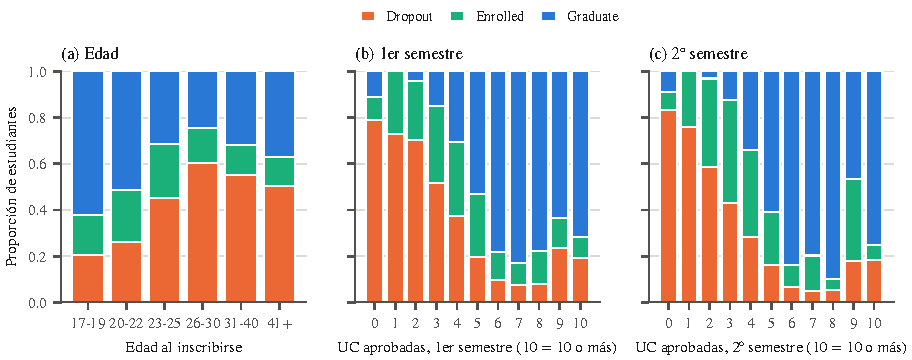
\includegraphics[width=\textwidth]{fig_eda_clases.pdf}
\caption{Composición de clases en Train según (a) la edad al inscribirse, (b) las UC aprobadas en el primer semestre y (c) las UC aprobadas en el segundo semestre (el último valor agrupa 10 o más). Cada barra suma 100\,\%; con cero UC aprobadas predomina la deserción.}
\label{fig:eda}
\end{figure*}

\textbf{Valores atípicos.} La edad al inscribirse va de \edadMin{} a \edadMax{} años y \nOutEdad{} estudiantes (\pOutEdad\,\%) quedan fuera de los límites de la regla del rango intercuartílico. Se conservaron: son valores reales de un segmento con un comportamiento distinto (el de 26 a 30 años), y eliminarlos quitaría información sin que los modelos de árboles lo requieran; para RL y SVM el escalado acota su influencia.

\textbf{Codificación y escalado.} Un \texttt{ColumnTransformer} aplica \texttt{StandardScaler} a las \nNum{} numéricas, \emph{one-hot} a las \nNom{} nominales y deja pasar las \nBin{} binarias. El \emph{one-hot} usa \texttt{min\_frequency}=0.01 (las categorías con menos de 1\,\% se agrupan) y \texttt{handle\_unknown=infrequent\_if\_exist}, de modo que las \nCatOrig{} categorías originales quedan en \nOH{} columnas y el total de entrada es de \nCols{} columnas. El código de la licenciatura no tiene orden (su correlación lineal con \cD{} es de \rCurso{}), por lo que se codifica \emph{one-hot}.

\textbf{Correlaciones y selección de variables.} Hay \nCorrAlta{} pares de variables numéricas con $|r|>0.8$ de \nParesNum{} posibles, todos entre el primer y el segundo semestre (por ejemplo, UC aprobadas: $r=\rAprobSem$; inscritas: $r=\rInscSem$). No se eliminó ninguna variable: la penalización L1 de la RL, la regularización de las SVM y los árboles manejan la colinealidad, y seleccionar variables con el conjunto completo antes de partir es una fuente conocida de fuga \cite{kapoor2023}.

\textbf{Desbalance.} No se usó remuestreo sintético. Se emplearon pesos de clase balanceados (\texttt{class\_weight}) en los modelos que los admiten, \Fm{} como métrica principal de selección y, para la RL, una regla de decisión sobre $P(\mathrm{Dropout})$ con umbral elegido sobre predicciones fuera de bolsa (OOF) de Train. Con una razón de 2.8 a 1, el desbalance es moderado y los pesos evitan inventar estudiantes sintéticos \cite{chawla2002}.

\textbf{Control de fuga.} Todo ajuste (escalado, codificación, selección de hiperparámetros, umbral) ocurre solo con datos de entrenamiento: el preprocesamiento vive dentro de un \texttt{Pipeline} que se reajusta en cada fold, y las búsquedas se hacen con validación cruzada sobre Train. El único análisis posterior que usa Test para algo distinto de la evaluación es la importancia por permutación (Sec.~\ref{sec:grafico}), explícitamente \emph{a posteriori} y no usada para seleccionar nada.

\subsection{Modelos}
Se parte de la RL y las SVM de proyectos previos del curso y se agregan ensambles, siguiendo las descripciones de \cite{geron2019} e implementaciones de scikit-learn \cite{pedregosa2011}.

\textbf{Modelos de referencia.} \emph{Dummy} predice la clase mayoritaria y marca el piso (\Fm{} de \teFDUM{}). La \textbf{RL} multinomial con penalización L1 \cite{tibshirani1996} y solver \texttt{saga} \cite{defazio2014} es interpretable y es el modelo base del curso. Las \textbf{SVM} (lineal, polinomial y RBF) \cite{cortes1995} buscan el margen máximo y, con núcleos, fronteras no lineales; las probabilidades de la SVM se obtienen con escalamiento de Platt \cite{platt1999}.

\textbf{Ensambles de árboles.} Un árbol de decisión es el estimador base: de bajo sesgo pero de alta varianza. \textbf{Bagging} \cite{breiman1996} y \textbf{Pasting} \cite{breiman1999} promedian árboles entrenados con submuestras (con y sin reemplazo, respectivamente) para reducir la varianza; \textbf{Random Forest} \cite{breiman2001} agrega un sorteo de variables en cada división. \textbf{AdaBoost} \cite{freund1997} y \textbf{Gradient Boosting} \cite{friedman2001} entrenan árboles de forma secuencial para reducir el sesgo; \textbf{HistGradientBoosting} es la variante con histogramas de scikit-learn, inspirada en LightGBM \cite{ke2017}, mucho más rápida.

\textbf{Ensambles híbridos e interpretables.} \textbf{Voting} combina RL, SVM, Random Forest, Gradient Boosting y HistGradientBoosting por voto mayoritario (\emph{hard}) o por promedio de probabilidades (\emph{soft}). \textbf{Stacking} \cite{wolpert1992} entrena una RL balanceada sobre las predicciones fuera de fold de esos cinco modelos (las versiones base de ambos usan solo RL, SVM y Random Forest). La \textbf{EBM} (\emph{Explainable Boosting Machine}) \cite{lou2013,nori2019} es un modelo aditivo con interacciones por pares, entrenado por boosting cíclico: se incluye como alternativa interpretable de caja de cristal frente a los ensambles opacos.

\subsection{Diseño experimental}\label{sec:disenio}
\textbf{Partición y validación.} Una partición estratificada 80/20 con \texttt{random\_state}=42 da Train de \Ntr{} (\ntrD{}, \ntrE{} y \ntrG{} estudiantes de \cD, \cE{} y \cG) y Test de \Nte{} (\nteD{}, \nteE{} y \nteG{}). En Train se usa validación cruzada estratificada de 5 folds (\texttt{shuffle}, semilla 42), la misma para todos los modelos. La Fig.~\ref{fig:flujo} resume el flujo y separa tres usos de los datos: \emph{entrenamiento} (ajuste de cada modelo dentro de un fold), \emph{selección} (comparación de configuraciones con la validación cruzada) y \emph{evaluación final} (Test, una sola vez por modelo y sin reajustar nada).

\begin{figure*}[t]
\centering
\begin{tikzpicture}[font=\scriptsize, >=Stealth,
  caja/.style={draw=black!60, rounded corners=1.5pt, minimum height=9mm, align=center, text width=3.0cm, inner sep=2pt, fill=white},
  tr/.style={caja, fill=blue!7},
  te/.style={caja, fill=orange!14, draw=orange!70!black},
  fl/.style={->, thin, black!70}]
\node[tr] (ds) {Conjunto UCI 697\\ \Ntot{} estudiantes, 36 variables};
\node[tr, right=5mm of ds] (sp) {Partición estratificada 80/20\\ \texttt{random\_state}=42};
\node[tr, right=5mm of sp] (eda) {Train (\Ntr{}): análisis exploratorio\\ (solo Train)};
\node[tr, right=5mm of eda] (pipe) {\texttt{Pipeline}: escalado, \emph{one-hot} y modelo, reajustado en cada fold};
\node[tr, below=9mm of ds] (cv) {CV estratificada de 5 folds: modelos base};
\node[tr, right=5mm of cv] (bus) {Búsqueda de hiperparámetros (\Fm{}), mismos folds};
\node[tr, right=5mm of bus] (rep) {CV repetida 5$\times$5, Nadeau--Bengio y Holm};
\node[tr, right=5mm of rep] (fit) {Reajuste del modelo elegido con todo Train};
\node[te, below=9mm of fit] (test) {Test (\Nte{}): una evaluación por modelo; IC bootstrap, McNemar};
\draw[fl] (ds) -- (sp);
\draw[fl] (sp) -- (eda);
\draw[fl] (eda) -- (pipe);
\draw[fl] (pipe.south) -- ++(0,-4.5mm) -| (cv.north);
\draw[fl] (cv) -- (bus);
\draw[fl] (bus) -- (rep);
\draw[fl] (rep) -- (fit);
\draw[fl] (fit) -- (test);
\draw[fl, dashed, orange!70!black] (sp.north) -- ++(0,3.5mm) -| ($(test.east)+(4mm,0)$) -- (test.east);
\node[font=\scriptsize\itshape, orange!60!black, anchor=south west] at ($(sp.north)+(2mm,3.5mm)$) {Test se separa y no se toca hasta el final};
\end{tikzpicture}
\caption{Flujo experimental. En azul, los pasos que solo usan Train (entrenamiento y selección); en naranja, el único paso que usa Test. El preprocesamiento se ajusta dentro de cada fold para evitar fuga de información.}
\label{fig:flujo}
\end{figure*}

\textbf{Configuración base y optimización.} Cada modelo se evalúa primero con una configuración inicial razonable (Tabla~\ref{tab:base}; para RL y SVM, los parámetros por defecto de scikit-learn). Las versiones base de Voting y Stacking reutilizan la RL y la SVM RBF ya optimizadas en proyectos previos (con el mismo Train), por lo que no son ingenuas. Después se optimiza con \texttt{RandomizedSearchCV} o \texttt{GridSearchCV} \cite{bergstra2012}, con \Fm{} como puntaje, los mismos 5 folds y reajuste con la mejor combinación. La Tabla~\ref{tab:espacios} lista lo que se evaluó en cada búsqueda y la Tabla~\ref{tab:opt}, lo que se seleccionó. Como el mismo puntaje sirve para seleccionar y estimar, el de la mejor combinación es optimista \cite{cawley2010}; lo acotamos comparándolo con la validación cruzada repetida (Sec.~\ref{sec:grafico}).

\begin{table*}[t]
\caption{Hiperparámetros evaluados en cada búsqueda (todas con los mismos 5 folds estratificados, puntaje F1 macro y reajuste con el mejor).}
\label{tab:espacios}
\centering\scriptsize
\setlength{\tabcolsep}{3pt}
\begin{tabular}{@{}p{2.7cm}p{12.4cm}r@{}}
\toprule
Modelo & Hiperparámetros evaluados & Combinaciones \\
\midrule
Random Forest & \texttt{max\_features} \{sqrt, log2, 0.2, 0.35, 0.5\}; \texttt{min\_samples\_leaf} \{1, 2, 3, 5, 8, 12, 20\}; \texttt{max\_depth} \{None, 8, 12, 16\}; \texttt{class\_weight} \{None, balanced, balanced\_subsample\}; \texttt{criterion} \{gini, entropy\} & 40 (aleatoria) \\
Bagging y Pasting & \texttt{max\_samples} \{0.3, 0.5, 0.7, 1.0\} (Pasting: hasta 0.9); \texttt{max\_features} \{0.3, 0.6, 1.0\}; \texttt{max\_depth} \{4, 6, 8, 12, None\}; \texttt{min\_samples\_leaf} \{1, 5, 10, 20\}; \texttt{class\_weight} \{None, balanced\} del árbol & 30 + 30 (aleatoria) \\
AdaBoost & \texttt{n\_estimators} \{25, 50, 100, 200, 400\}; \texttt{learning\_rate} \{0.03, 0.1, 0.3, 1.0\}; \texttt{max\_depth} del árbol \{1, 2, 3, 4, 6, 8, 10\} & 140 (malla) \\
Gradient Boosting & \texttt{learning\_rate} \{0.02, 0.05, 0.1, 0.2\}; \texttt{n\_estimators} \{100, 200, 300\}; \texttt{max\_depth} \{2, 3, 4, 5\}; \texttt{subsample} \{0.5, 0.7, 1.0\}; \texttt{min\_samples\_leaf} \{1, 5, 10, 20\}; \texttt{max\_features} \{None, sqrt, 0.3\} & 30 (aleatoria) \\
HistGradientBoosting & \texttt{learning\_rate} \{0.02, 0.05, 0.1, 0.2\}; \texttt{max\_iter} \{100, 200, 400\}; \texttt{max\_leaf\_nodes} \{7, 15, 31\}; \texttt{min\_samples\_leaf} \{10, 20, 40, 80\}; \texttt{l2\_regularization} \{0, 1, 10\}; \texttt{max\_depth} \{None, 3, 5\}; \texttt{class\_weight} \{None, balanced\} & 40 (aleatoria) \\
EBM & \texttt{interactions} \{0, 10, 20\}; \texttt{learning\_rate} \{0.01, 0.03\}; \texttt{max\_leaves} \{2, 3\}; \texttt{min\_samples\_leaf} \{4, 20\} & 24 (malla) \\
Voting & pesos de (RL, SVM, RF, GB, HGB) $\in$ \{(1,1,1,1,1), (1,1,2,2,2), (2,1,1,1,1), (1,1,1,2,2), (1,0,1,1,1)\} & 5 (malla) \\
Stacking & $C$ del meta-modelo (regresión logística balanceada) $\in$ \{0.01, 0.1, 1, 10\}, con validación cruzada interna de 5 folds & 4 \\
RL y SVM & heredados de proyectos previos del curso (búsquedas sobre el mismo Train); aquí se usan fijos & --- \\
\bottomrule
\end{tabular}
\end{table*}


\textbf{Métricas.} La métrica principal es el F1 macro, el promedio sin ponderar de los F1 de las tres clases (ec.~\ref{eq:f1}), porque da el mismo peso a la clase minoritaria \cE:
\begin{equation}
F1_{\mathrm{macro}}=\frac13\sum_{c\in\{\mathrm{D},\mathrm{E},\mathrm{G}\}}\frac{2\,P_c R_c}{P_c+R_c}.
\label{eq:f1}
\end{equation}
Se reportan también exactitud, precisión y exhaustividad macro, F1 ponderado, el coeficiente de correlación de Matthews (MCC) \cite{matthews1975}, $\kappa$ de Cohen \cite{cohen1960} y AUC ROC uno contra el resto \cite{fawcett2006}. La exactitud se complementa con las demás porque favorece a la clase mayoritaria; MCC y $\kappa$ resumen la tabla de confusión completa.

\textbf{Inferencia.} Para comparar un modelo con la RL se usan tres herramientas. (a) Validación cruzada repetida de 5$\times$5 con la prueba $t$ corregida de Nadeau y Bengio \cite{nadeau2003}, cuyo estadístico (ec.~\ref{eq:nb}) para las diferencias $d_j$ de $J=25$ remuestreos es
\begin{equation}
t=\frac{\bar d}{\sqrt{\left(\tfrac1J+\tfrac{n_2}{n_1}\right)\hat\sigma_d^2}},\qquad \tfrac{n_2}{n_1}=\tfrac14,
\label{eq:nb}
\end{equation}
con ajuste de Holm \cite{holm1979} por las comparaciones: si los $m$ $p$-valores ordenados son $p_{(1)}\le\dots\le p_{(m)}$, el ajustado es $\tilde p_{(i)}=\max_{j\le i}\min\{1,(m-j+1)p_{(j)}\}$. (b) En Test, intervalos de 95\,\% por bootstrap \cite{efron1979} con 2,000 remuestreos de los \Nte{} estudiantes y diferencias pareadas con las mismas remuestras. (c) La prueba exacta de McNemar \cite{mcnemar1947} sobre los aciertos de cada par de modelos.

\textbf{Herramientas y reproducibilidad.} Python 3.14.8, scikit-learn 1.9.1, pandas 2.3.3, NumPy 2.5.4 e interpret 0.7.8 (EBM). Semilla 42 en la partición, los folds y los modelos. El código, los cuadernos ejecutados y las instrucciones para reproducir los resultados están en \expandafter\url\expandafter{\repoURL}.

%=====================================================================================================================
\section{Resultados y discusión}\label{sec:res}

\subsection{Modelos base}
La Tabla~\ref{tab:base} muestra los modelos con su configuración inicial, evaluados con validación cruzada. La mejor \Fm{} base es la de Gradient Boosting (\cvFGBB), seguida de Voting (hard) (\cvFVHB), EBM (\cvFEBMB) y Voting (soft) (\cvFVSB); todas superan a la RL por defecto (\cvFLRD) y, por mucho, a Dummy (\cvFDUM). Un solo árbol (\cvFDT) rinde bastante menos que sus versiones de ensamble: Bagging (\cvFBAGB), Pasting (\cvFPASB) y Random Forest (\cvFRFB), lo que confirma el efecto de reducir la varianza. Las SVM polinomial y RBF con parámetros por defecto quedan por debajo de la RL (\cvFSVPD{} y \cvFSVRD{}) y con brechas grandes entre entrenamiento y validación (\cvGapSVPD{} y \cvGapSVRD{}), señal de sobreajuste por una configuración no ajustada. Random Forest y Gradient Boosting memorizan Train (brechas de \cvGapRFB{} y \cvGapGBB{}) y aun así están entre los mejores en validación, de modo que una brecha grande no implica por sí sola peor generalización; la de AdaBoost (\cvGapADAB) es mínima solo porque su configuración base se detuvo en 10 estimadores.

\begin{table*}[t]
\caption{Modelos base evaluados con validación cruzada estratificada de 5 folds sobre Train (media; F1 macro con desviación entre folds). La brecha es el F1 de entrenamiento menos el F1 de validación. Negritas: mejor F1 macro (sin contar a Dummy).}
\label{tab:base}
\centering\scriptsize
\setlength{\tabcolsep}{3pt}
\begin{tabular}{@{}p{2.9cm}p{7.6cm}ccccc@{}}
\toprule
Modelo & Configuración inicial & Acc. & F1 macro & MCC & AUC & Brecha \\
\midrule
Dummy & predice la clase mayoritaria & 0.499 & 0.222$\pm$0.000 & 0.000 & 0.500 & 0.000 \\
Regresión logística & parámetros por defecto de scikit-learn & 0.776 & 0.701$\pm$0.019 & 0.629 & 0.889 & 0.039 \\
SVM lineal & ídem (\texttt{LinearSVC}) & 0.772 & 0.681$\pm$0.017 & 0.623 & 0.872 & 0.038 \\
SVM polinomial & ídem (\texttt{SVC}, grado 3) & 0.752 & 0.664$\pm$0.020 & 0.590 & 0.850 & 0.137 \\
SVM RBF & ídem (\texttt{SVC}, RBF) & 0.772 & 0.691$\pm$0.025 & 0.623 & 0.861 & 0.103 \\
Árbol de decisión & profundidad 8, \texttt{min\_samples\_leaf}=10, balanceado & 0.692 & 0.656$\pm$0.020 & 0.525 & 0.836 & 0.087 \\
Voting (hard) & voto mayoritario de la RL ($C$=0.3, L1) y la SVM RBF ($C$=100, $\gamma$=0.001) ya optimizadas, y un Random Forest de 200 árboles & 0.780 & 0.729$\pm$0.018 & 0.640 & --- & 0.077 \\
Voting (soft) & promedio de probabilidades de los mismos tres (SVM calibrada con Platt) & 0.790 & 0.726$\pm$0.018 & 0.652 & 0.897 & 0.052 \\
Bagging & 200 árboles (el anterior) con remuestreo, \texttt{max\_samples}=0.5 & 0.747 & 0.702$\pm$0.013 & 0.596 & 0.876 & 0.052 \\
Pasting & 200 árboles (el anterior) sin reemplazo, \texttt{max\_samples}=0.5 & 0.743 & 0.700$\pm$0.016 & 0.593 & 0.877 & 0.065 \\
Random Forest & 300 árboles, \texttt{sqrt}, \texttt{min\_samples\_leaf}=5, \texttt{balanced\_subsample} & 0.766 & 0.718$\pm$0.022 & 0.620 & 0.886 & 0.146 \\
AdaBoost & 200 estimadores, $\eta$=0.5, árboles de profundidad 2 (se detuvo en 10) & 0.727 & 0.678$\pm$0.013 & 0.562 & 0.854 & 0.006 \\
Gradient Boosting & 200 iteraciones, $\eta$=0.1, profundidad 3, \texttt{subsample}=0.8, pesos balanceados & 0.771 & \textbf{0.730$\pm$0.021} & 0.634 & 0.893 & 0.167 \\
HistGradientBoosting & 200 iteraciones, $\eta$=0.1, 15 hojas, balanceado & 0.770 & 0.716$\pm$0.016 & 0.624 & 0.890 & 0.282 \\
Stacking & los mismos tres $\rightarrow$ RL balanceada (5 folds internos) & 0.759 & 0.722$\pm$0.021 & 0.623 & 0.896 & 0.083 \\
EBM (GAM) & modelo aditivo sin interacciones (\texttt{interactions}=0) & 0.752 & 0.714$\pm$0.018 & 0.610 & 0.885 & 0.043 \\
EBM & 10 interacciones de a pares & 0.766 & 0.728$\pm$0.009 & 0.631 & 0.892 & 0.057 \\
\bottomrule
\end{tabular}
\end{table*}


\subsection{Modelos optimizados}
La Tabla~\ref{tab:opt} compara cada modelo con su versión base, tanto en validación cruzada como en Test, y la Fig.~\ref{fig:antes} muestra el efecto en validación.

\begin{table*}[t]
\caption{Modelos optimizados: hiperparámetros seleccionados, F1 macro en validación cruzada (CV, 5 folds sobre Train) y en Test, frente a los mismos modelos con su configuración inicial (``base''; para RL y SVM, los parámetros por defecto). $\Delta$ = optimizado $-$ base.}
\label{tab:opt}
\centering\scriptsize
\setlength{\tabcolsep}{3pt}
\begin{tabular}{@{}p{2.6cm}p{6.5cm}cccccc@{}}
\toprule
 & & \multicolumn{3}{c}{F1 macro en CV} & \multicolumn{3}{c}{F1 macro en Test} \\
\cmidrule(lr){3-5}\cmidrule(lr){6-8}
Modelo & Hiperparámetros seleccionados & Base & Optimizado & $\Delta$ & Base & Optimizado & $\Delta$ \\
\midrule
RL & penalización L1 (\texttt{saga}), $C$=0.3, balanceada & 0.701 & 0.717$\pm$0.019 & +0.016 & 0.699 & 0.688 & $-$0.011 \\
SVM lineal & $C$=0.01, balanceada & 0.681 & 0.709$\pm$0.019 & +0.028 & 0.670 & 0.708 & +0.038 \\
SVM polinomial & grado 2, \texttt{coef0}=1, $C$=1, balanceada & 0.664 & 0.721$\pm$0.011 & +0.057 & 0.631 & 0.696 & +0.065 \\
SVM RBF & $C$=100, $\gamma$=0.001 & 0.691 & 0.722$\pm$0.011 & +0.031 & 0.693 & 0.690 & $-$0.003 \\
Random Forest & \texttt{min\_samples\_leaf}=2, \texttt{log2}, profundidad 16, entropy, balanceada & 0.718 & 0.726$\pm$0.022 & +0.009 & 0.698 & 0.716 & +0.018 \\
Bagging & \texttt{max\_samples}=1, \texttt{max\_features}=0.3, árbol de profundidad 12 y \texttt{min\_samples\_leaf}=5, balanceado & 0.702 & 0.710$\pm$0.019 & +0.008 & 0.684 & 0.713 & +0.029 \\
Pasting & \texttt{max\_samples}=0.9, \texttt{max\_features}=0.3, árbol de profundidad 12 y \texttt{min\_samples\_leaf}=5, balanceado & 0.700 & 0.719$\pm$0.020 & +0.018 & 0.680 & 0.710 & +0.029 \\
AdaBoost & árboles de profundidad 6, $\eta$=0.1, 50 estimadores & 0.678 & 0.718$\pm$0.019 & +0.039 & 0.677 & 0.677 & +0.001 \\
Gradient Boosting & $\eta$=0.05, 300 iteraciones, profundidad 4, \texttt{subsample}=0.7, \texttt{max\_features}=0.3, hoja mínima 5 & 0.730 & 0.732$\pm$0.019 & +0.002 & 0.692 & 0.687 & $-$0.005 \\
HistGradientBoosting & $\eta$=0.1, 100 iteraciones, 15 hojas, hoja mínima 10, $\lambda_2$=1, balanceado & 0.716 & 0.734$\pm$0.019 & +0.018 & 0.683 & 0.675 & $-$0.008 \\
EBM & 10 interacciones, $\eta$=0.03, 3 hojas, hoja mínima 4 & 0.728 & 0.731$\pm$0.014 & +0.002 & 0.695 & 0.697 & +0.002 \\
Voting (hard) & pesos (RL, SVM, RF, GB, HGB) = (1, 1, 2, 2, 2) & 0.729 & 0.737$\pm$0.019 & +0.008 & 0.699 & 0.693 & $-$0.006 \\
Voting (soft) & pesos (RL, SVM, RF, GB, HGB) = (1, 1, 2, 2, 2) & 0.726 & 0.737$\pm$0.022 & +0.012 & 0.700 & 0.703 & +0.003 \\
Stacking & 5 modelos base (RL, SVM, RF, GB, HGB) $\rightarrow$ RL balanceada & 0.722 & 0.733$\pm$0.018 & +0.011 & 0.702 & 0.697 & $-$0.005 \\
\bottomrule
\end{tabular}
\end{table*}


\begin{figure}[t]
\centering
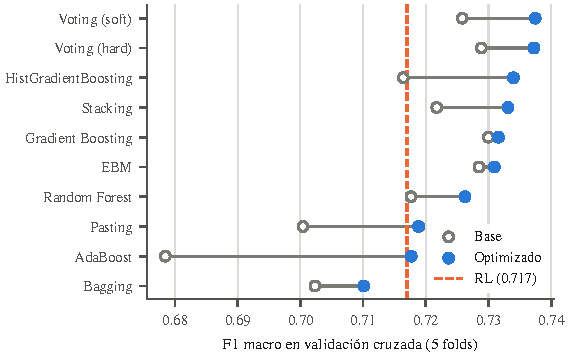
\includegraphics[width=\columnwidth]{fig_antes_despues.pdf}
\caption{\Fm{} en validación cruzada de 5 folds antes (círculo vacío) y después (círculo lleno) de optimizar. La línea punteada marca la RL optimizada.}
\label{fig:antes}
\end{figure}

\textbf{Validación.} Los \nOptMejoraCV{} ensambles mejoran en validación, de \dcvMin{} a \dcvMax{} (promedio \dcvMedia{}). La mayor ganancia, la de AdaBoost (\dcvADA), se debe sobre todo a que su configuración inicial era débil, no a una ventaja intrínseca de la búsqueda. Las SVM ganan entre \dcvSVL{} y \dcvSVP{} porque sus valores por defecto eran pobres, y la RL gana \dcvLR{}. Tras optimizar, las \Fm{} de los modelos optimizados quedan en un rango estrecho (\cvFMinOpt{} a \cvFMaxOpt{}) comparable a la desviación entre folds (0.011 a 0.022).

\textbf{Test.} En Test solo \nOptMejoraTest{} de los diez ensambles mejoran, con una ganancia media de \dteMedia{}: Bagging y Pasting suben \dteBAG{} y \dtePAS{} y Random Forest \dteRF{}, mientras que Gradient Boosting, HistGradientBoosting, Voting (hard) y Stacking quedan por debajo de su versión base (de $-$0.005 a $-$0.008, dentro del ruido de un intervalo de unos $\pm0.03$). La RL optimizada baja en Test (\dteLR{}) aunque sube en validación: su exactitud cae de \teAccLRD{} (por defecto) a \teAccLR{}, porque optimizar por \Fm{} con pesos balanceados cambió exactitud por exhaustividad de \cE{} (de \reELRD{} a \reELR). En síntesis, la ganancia de la optimización en validación (\dcvMedia{}) no se traslada de forma confiable a Test (\dteMedia{}).

\begin{table*}[t]
\caption{Evaluación final en Test ($n=885$, evaluada una sola vez por modelo). Precisión, exhaustividad y F1 son promedios macro; entre corchetes, el intervalo de confianza de 95\,\% por bootstrap (2{,}000 remuestreos de los 885 estudiantes) del F1 macro, calculado para los modelos que se compararon formalmente. Negritas: mejor valor de la columna (sin contar a Dummy).}
\label{tab:test}
\centering\scriptsize
\setlength{\tabcolsep}{3pt}
\begin{tabular}{@{}lcccccccc@{}}
\toprule
Modelo & Acc. & Prec. & Exh. & F1 macro [IC 95\,\%] & F1 pond. & MCC & $\kappa$ & AUC \\
\midrule
Dummy (clase mayoritaria) & 0.499 & 0.166 & 0.333 & 0.222  & 0.333 & 0.000 & 0.000 & 0.500 \\
Regresión logística (RL) & 0.727 & 0.697 & 0.700 & 0.688 [0.656, 0.719] & 0.740 & 0.576 & 0.570 & 0.884 \\
RL + regla $P(\mathrm{Dropout})\geq0.40$ & 0.725 & 0.687 & 0.691 & 0.683 [0.651, 0.712] & 0.737 & 0.570 & 0.566 & 0.884 \\
SVM lineal & \textbf{0.768} & 0.717 & 0.702 & 0.708  & 0.765 & \textbf{0.620} & \textbf{0.618} & 0.872\textsuperscript{a} \\
SVM polinomial & 0.734 & 0.703 & 0.707 & 0.696  & 0.746 & 0.586 & 0.581 & 0.862\textsuperscript{a} \\
SVM RBF & 0.763 & 0.705 & 0.682 & 0.690 [0.657, 0.722] & 0.754 & 0.607 & 0.604 & 0.853\textsuperscript{a} \\
Voting (hard) & 0.739 & 0.697 & 0.700 & 0.693 [0.659, 0.723] & 0.749 & 0.589 & 0.586 & --- \\
Voting (soft) & 0.756 & 0.705 & 0.704 & 0.703 [0.669, 0.734] & 0.759 & 0.606 & 0.605 & \textbf{0.890} \\
Bagging & 0.762 & 0.716 & 0.715 & 0.713 [0.680, 0.743] & 0.765 & 0.616 & 0.615 & 0.882 \\
Pasting & 0.755 & 0.711 & 0.714 & 0.710 [0.677, 0.740] & 0.761 & 0.608 & 0.606 & 0.884 \\
Random Forest & 0.759 & \textbf{0.721} & \textbf{0.721} & \textbf{0.716} [0.683, 0.747] & \textbf{0.766} & 0.617 & 0.614 & 0.887 \\
AdaBoost & 0.714 & 0.692 & 0.689 & 0.677 [0.645, 0.708] & 0.729 & 0.559 & 0.551 & 0.874 \\
Gradient Boosting & 0.729 & 0.693 & 0.697 & 0.687 [0.655, 0.717] & 0.742 & 0.578 & 0.573 & 0.887 \\
HistGradientBoosting & 0.727 & 0.678 & 0.679 & 0.675 [0.641, 0.705] & 0.734 & 0.564 & 0.562 & 0.875 \\
Stacking & 0.738 & 0.703 & 0.707 & 0.697 [0.664, 0.727] & 0.750 & 0.592 & 0.587 & 0.888 \\
EBM & 0.731 & 0.705 & 0.712 & 0.697 [0.665, 0.725] & 0.745 & 0.587 & 0.579 & 0.889 \\
\bottomrule
\end{tabular}

\vspace{2pt}
\raggedright\scriptsize\textsuperscript{a}\,AUC calculada con \texttt{decision\_function} de scikit-learn; con probabilidades (\texttt{libsvm}) la SVM RBF obtiene 0.884, igual que la RL. Voting (hard) no produce puntajes. Sin IC: modelos que no entraron al bootstrap.
\end{table*}


La Tabla~\ref{tab:test} reúne la evaluación final. Salvo Dummy, las \Fm{} de los modelos optimizados quedan entre \testFMin{} y \testFMax{}; el mejor valor puntual es el de Random Forest (\teFRF, IC 95\,\% [\teLoRF, \teHiRF]), seguido de Bagging (\teFBAG) y Pasting (\teFPAS); los tres difieren en \rangoTresTest{} y sus intervalos se solapan casi por completo. La SVM lineal, un modelo sencillo, tiene la mayor exactitud (\teAccSVL), el mayor MCC (\teMccSVL) y un \Fm{} de \teFSVL{}, es decir, los ensambles no dominan en todas las métricas. Voting (soft) tiene el mayor AUC (\teAucVS).

\textbf{Comparaciones pareadas en Test.} La Tabla~\ref{tab:pareadas} compara cada modelo con la RL con su regla de decisión (el modelo final del proyecto previo, \Fm{} de \teFLRR{}). Hay tres lecturas. (i) \emph{\Fm{}, el criterio principal:} solo Random Forest (\parRF) y Bagging (\parBAG) tienen intervalos que excluyen el cero, y apenas; Voting (soft) difiere en \parVSF{}, con el cero dentro del intervalo. (ii) \emph{Exactitud y McNemar:} cuatro modelos (SVM RBF, Voting (soft), Bagging y Random Forest) aciertan significativamente más estudiantes que la RL con regla incluso tras el ajuste de Holm ($p$ ajustado de \phoSVR{} a \phoRF{}); por ejemplo, Voting (soft) acierta donde la RL falla en 55 casos y la RL donde Voting (soft) falla en 28. Pero esa ventaja es compatible con un punto de operación distinto: la RL con regla se ajustó para detectar \cE{} y desertores y tiene una exactitud de \teAccLRR{}, mientras que la RL por defecto, sin ese ajuste, llega a \accLRD{} (más que cualquier modelo de la Tabla~\ref{tab:test}) con una exhaustividad de \cE{} de solo \reELRD. (iii) \emph{AUC,} que no depende del umbral: ninguna diferencia con la RL es detectable en los modelos con probabilidades (de \auMin{} a \auMax{}, todas con el cero dentro del intervalo); la de la SVM RBF es un artefacto de cómo se calculó (nota de la tabla). Además, McNemar condiciona a los modelos ya ajustados y no recoge la variabilidad por el entrenamiento \cite{dietterich1998}, y los intervalos bootstrap de la tabla no están corregidos por multiplicidad: los leemos como indicios, no como confirmaciones.

\begin{table*}[t]
\caption{Diferencias pareadas en Test frente a la RL con su regla de decisión (modelo final del proyecto previo): diferencia observada e intervalo de 95\,\% por bootstrap pareado (2,000 remuestreos; sin corrección por multiplicidad). McNemar: estudiantes que acierta solo el modelo / solo la RL, $p$ exacto y $p$ ajustado por Holm sobre 11 comparaciones (negritas: $<0.05$).}
\label{tab:pareadas}
\centering\scriptsize
\setlength{\tabcolsep}{3pt}
\begin{tabular}{@{}lccccccc@{}}
\toprule
Modelo & $\Delta$F1 macro & $\Delta$ exactitud & $\Delta$MCC & $\Delta$AUC & Solo él / solo RL & $p$ McNemar & $p$ Holm \\
\midrule
Random Forest & +0.033 [+0.006, +0.060] & +0.034 [+0.011, +0.058] & +0.046 [+0.010, +0.082] & +0.003 [$-$0.007, +0.015] & 70 / 40 & 0.005 & \textbf{0.044} \\
Bagging & +0.030 [+0.001, +0.059] & +0.036 [+0.011, +0.061] & +0.046 [+0.008, +0.085] & $-$0.002 [$-$0.014, +0.010] & 77 / 45 & 0.005 & \textbf{0.043} \\
Pasting & +0.026 [$-$0.002, +0.054] & +0.029 [+0.006, +0.053] & +0.038 [+0.001, +0.074] & +0.000 [$-$0.011, +0.012] & 72 / 46 & 0.021 & 0.147 \\
Voting (soft) & +0.020 [$-$0.005, +0.043] & +0.030 [+0.010, +0.051] & +0.035 [+0.004, +0.066] & +0.006 [$-$0.002, +0.014] & 55 / 28 & 0.004 & \textbf{0.040} \\
Stacking & +0.014 [$-$0.010, +0.036] & +0.012 [$-$0.008, +0.032] & +0.021 [$-$0.011, +0.051] & +0.004 [$-$0.003, +0.012] & 46 / 35 & 0.266 & 1.000 \\
EBM & +0.013 [$-$0.011, +0.036] & +0.006 [$-$0.016, +0.026] & +0.017 [$-$0.017, +0.047] & +0.005 [$-$0.004, +0.015] & 50 / 45 & 0.682 & 1.000 \\
Voting (hard) & +0.010 [$-$0.015, +0.032] & +0.014 [$-$0.008, +0.035] & +0.018 [$-$0.015, +0.050] & --- & 52 / 40 & 0.251 & 1.000 \\
SVM RBF & +0.007 [$-$0.020, +0.035] & +0.037 [+0.014, +0.061] & +0.037 [+0.001, +0.071] & $-$0.031 [$-$0.044, $-$0.018]\textsuperscript{a} & 72 / 39 & 0.002 & \textbf{0.025} \\
Gradient Boosting & +0.004 [$-$0.022, +0.029] & +0.003 [$-$0.020, +0.025] & +0.008 [$-$0.027, +0.042] & +0.003 [$-$0.007, +0.012] & 55 / 52 & 0.847 & 1.000 \\
AdaBoost & $-$0.006 [$-$0.034, +0.022] & $-$0.011 [$-$0.036, +0.012] & $-$0.011 [$-$0.050, +0.026] & $-$0.010 [$-$0.025, +0.005] & 59 / 69 & 0.426 & 1.000 \\
HistGradientBoosting & $-$0.008 [$-$0.037, +0.018] & +0.001 [$-$0.024, +0.024] & $-$0.006 [$-$0.045, +0.029] & $-$0.009 [$-$0.020, +0.002] & 59 / 58 & 1.000 & 1.000 \\
\bottomrule
\multicolumn{8}{@{}l}{\textsuperscript{a}\,AUC de la SVM calculada con \texttt{decision\_function}; con probabilidades no difiere de la RL (0.884 en ambas). El Voting (hard) no produce puntajes.}
\end{tabular}
\end{table*}


\subsection{Comparación con el estado del arte}\label{sec:sota}
La Tabla~\ref{tab:sota} resume los cinco estudios que usan el mismo conjunto de datos, con sus condiciones, y agrega el contexto de Martins et al.\ \cite{martins2023} y nuestros resultados.

\begin{table*}[t]
\caption{Trabajos que usan el mismo conjunto de datos (tres clases). Las condiciones experimentales difieren, por lo que las cifras no son directamente comparables (Sec.~\ref{sec:sota}). Los resultados de cada estudio se listan en el orden de sus modelos.}
\label{tab:sota}
\centering\scriptsize
\setlength{\tabcolsep}{3pt}
\renewcommand{\arraystretch}{1.12}
\begin{tabular}{@{}p{2.55cm}p{3.1cm}p{4.3cm}p{2.2cm}p{4.3cm}@{}}
\toprule
Autores (año) & Modelos & Datos y partición & Métrica & Resultado \\
\midrule
Praptomo et al.\ (2026) \cite{praptomo2026} & RL / RF / XGBoost (búsqueda aleatoria, 15 conf.) & UCI, 4,424; 80/20 estratificada (3,539/885), semilla 42; sin remuestreo & F1 macro & 0.683 / 0.698 / 0.701 (exactitud 0.768 / 0.772 / 0.761) \\
\addlinespace[2pt]
Nashier et al.\ (2026) \cite{nashier2026} & RL, RF, SVM RBF, XGBoost, LightGBM, CatBoost, apilado de los tres últimos & UCI, 4,424; 80/20 estratificada (3,539/885), semilla 42; malla con CV de 5 folds; sin remuestreo & F1 macro (Test) & 0.703 / 0.704 / 0.693 / 0.718 / 0.703 / 0.690 / 0.697 (IC 95\,\% del apilado: 0.663--0.729) \\
\addlinespace[2pt]
Villar y de Andrade (2024) \cite{villar2024} & SVM, RF, GB, XGBoost, CatBoost, LightGBM & UCI, 4,424; SMOTE; partición y folds no reportados & F1 por clase (media de las tres, calculada por nosotros) & 0.743 / 0.840 / 0.813 / 0.857 / 0.850 / 0.853 \\
\addlinespace[2pt]
Putra et al.\ (2025) \cite{putra2025} & RF / XGBoost & 4,424 (tras limpieza); 80/20 sin semilla ni estratificación reportadas; selección de 25 variables por correlación & Exactitud; sensibilidad & 0.806 / 0.790; 0.724 / 0.717 (F1 no reportado) \\
\addlinespace[2pt]
Wijiyanto et al.\ (2026) \cite{wijiyanto2026} & Apilado HLR-STACK (XGBoost + CatBoost + LightGBM $\rightarrow$ RL) & 4,424; 80/20 (tamaño y estratificación no reportados), CV de 7 folds, SMOTE en los folds, RFE & Exactitud; F1 (promedio no especificado); AUC & 0.844; 0.725; 0.915 \\
\addlinespace[2pt]
\emph{Contexto:} Martins et al.\ (2023) \cite{martins2023} & SVMSMOTE + RF / Balanced RF & Versión previa (4,433); 90/10, 10 repeticiones; fin del 1.\textsuperscript{er} semestre & F1 global (ponderado) & 0.745 / 0.744 \\
\addlinespace[2pt]
\textbf{Este trabajo} & RL con su regla / SVM lineal / Random Forest / Voting (soft) & UCI, 4,424; 80/20 estratificada (3,539/885), semilla 42; CV de 5 folds; Pipeline sin fuga & F1 macro (Test) & 0.683 / 0.708 / 0.716 / 0.703 (exactitud 0.725 / 0.768 / 0.759 / 0.756) \\
\bottomrule
\end{tabular}
\end{table*}


\textbf{Estudios con la misma partición.} Praptomo et al.\ \cite{praptomo2026} y Nashier et al.\ \cite{nashier2026} usan la misma partición 80/20 (\Ntr{}/\Nte{}) con semilla 42 y no remuestrean. Sus F1 macro en Test (0.683--0.718) y los nuestros (\testFMin{}--\testFMax{}) están en el mismo rango y sus diferencias son menores que la incertidumbre: el intervalo de 95\,\% del apilamiento de Nashier et al.\ (0.663--0.729) es del ancho de los nuestros (por ejemplo, [\teLoRF, \teHiRF] para Random Forest). Por eso no podemos ordenar los trabajos. Además, ellos seleccionan con una malla o una búsqueda propias, y los modelos no son los mismos (XGBoost, LightGBM y CatBoost frente a Random Forest, HistGradientBoosting y EBM aquí).

\textbf{Estudios con cifras más altas.} Villar y de Andrade (F1 por clase, con SMOTE y partición no reportada), Putra et al.\ (exactitud de 0.806, con selección de variables por correlación antes de partir y una composición de Test distinta) y Wijiyanto et al.\ (exactitud de 0.844, con SMOTE y RFE) reportan cifras más altas que las nuestras (exactitud de \teAccRF{} y \Fm{} de \teFRF{} para Random Forest). Esas diferencias coinciden con diferencias de protocolo que suelen inflar la métrica: remuestreo o selección de variables que, si se hacen antes de partir, filtran información de Test \cite{kapoor2023}; particiones o composiciones de Test distintas; y métricas distintas (exactitud o F1 por clase frente a F1 macro). En el caso de Wijiyanto et al.\ el artículo no permite determinar con claridad si el preprocesamiento precedió a la partición ni cómo se promedió el F1; no podemos afirmar si esa es la causa. De Martins et al.\ no hay comparación posible: usan otra versión de los datos, otra partición (90/10 con repeticiones) y el F1 ponderado al final del primer semestre.

\textbf{Conclusión de la comparación.} Con estas condiciones, \emph{no} afirmamos que nuestros modelos superen ni queden por debajo de los publicados: solo los de Praptomo et al.\ y Nashier et al.\ comparten partición y métrica con nosotros, y con ellos la evidencia es de equivalencia dentro del ruido.

\subsection{Análisis gráfico}\label{sec:grafico}
\textbf{Incertidumbre en Test.} La Fig.~\ref{fig:testic} dibuja el \Fm{} en Test con su intervalo bootstrap de 95\,\%. Los intervalos miden unos 0.06 de ancho y se solapan ampliamente: la diferencia entre el mejor y el peor de los trece modelos con intervalo es menor que lo que mide uno solo. Con \Nte{} estudiantes, el orden de la Tabla~\ref{tab:test} no es estable.

\begin{figure}[t]
\centering
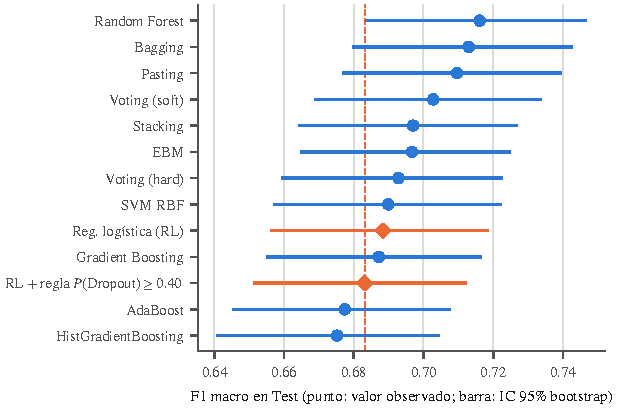
\includegraphics[width=\columnwidth]{fig_test_ic.pdf}
\caption{\Fm{} en Test (punto) con intervalo de 95\,\% por bootstrap (barra) para los modelos con intervalo; en naranja, la RL. La línea punteada marca la RL con regla.}
\label{fig:testic}
\end{figure}

\textbf{Validación cruzada repetida.} La Fig.~\ref{fig:cvrep} muestra la diferencia de \Fm{} frente a la RL en 5$\times$5 remuestreos. Voting (soft) es el mejor: \rvDVS{} (IC 95\,\% corregido [\rvLoVS, \rvHiVS], gana en \rvGVS{} de 25 remuestreos, $p=\rvPVS$), seguido de Voting (hard) (\rvDVH, $p=\rvPVH$) y Stacking (\rvDSTK). Pero con \nCompCV{} comparaciones, tras el ajuste de Holm el $p$ de Voting (soft) es \rvHVS{}: ninguno de los modelos es significativamente mejor que la RL (dos lo serían sin corregir). Los \Fm{} medios de este esquema (\rcFLR{} para la RL y \rcFVS{} para Voting (soft)) difieren de los de 5 folds en a lo sumo \optMaxAbs{} en los doce modelos optimizados, de modo que el optimismo de la selección es pequeño.

\begin{figure}[t]
\centering
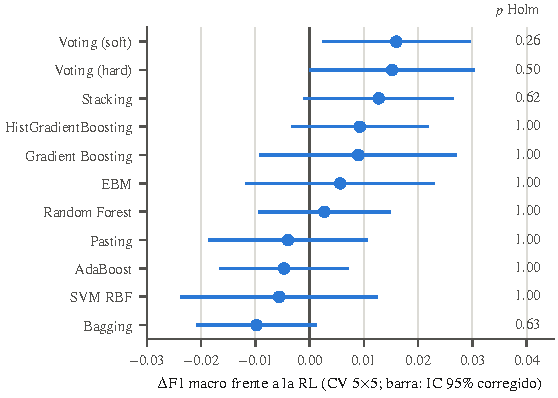
\includegraphics[width=\columnwidth]{fig_cv_repetida.pdf}
\caption{Diferencia de \Fm{} frente a la RL en validación cruzada repetida 5$\times$5 (punto: media; barra: IC 95\,\% con la corrección de Nadeau y Bengio). A la derecha, el $p$ de Holm; ninguna diferencia es significativa tras el ajuste.}
\label{fig:cvrep}
\end{figure}

\textbf{De validación a Test.} La Fig.~\ref{fig:gen} muestra para cada modelo optimizado el \Fm{} de entrenamiento, de validación y de Test. Entrenamiento va de \trainFMin{} a \trainFMax{}, y de validación a Test los modelos pierden en promedio \perdidaMedia{} (de \perdidaMin{} a \perdidaMax{}). El orden de validación no predice el de Test: entre los \nEnsGen{} ensambles, la correlación de Spearman entre ambos es de \rhoCVTest{} ($p=\pCVTest$), y la brecha de entrenamiento tampoco explica la pérdida ($\rho=\rhoGap$, $p=\pGap$). Dado que los \Fm{} de validación abarcan solo 0.027 puntos, esto es lo esperable si las diferencias entre modelos están en el ruido.

\begin{figure}[t]
\centering
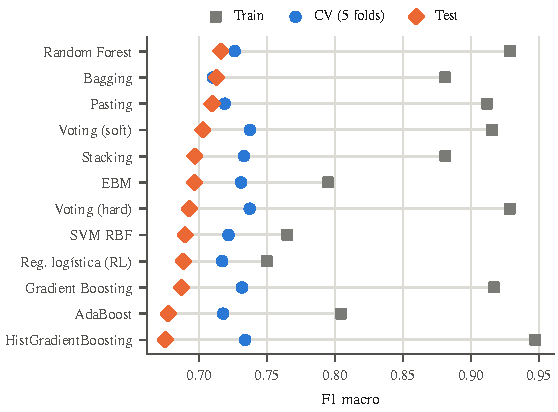
\includegraphics[width=\columnwidth]{fig_generalizacion.pdf}
\caption{\Fm{} de entrenamiento (cuadrado), validación cruzada (círculo) y Test (rombo) de los modelos optimizados.}
\label{fig:gen}
\end{figure}

\textbf{Errores por clase.} La Fig.~\ref{fig:conf} y la Tabla~\ref{tab:clases} muestran dónde se equivocan los modelos. \cG{} es la clase más fácil (F1 de 0.82 a 0.86) y \cD{} queda en 0.75--0.77; el límite está en \cE{} (F1 de 0.45 a 0.53), que se confunde con las otras dos. Los modelos difieren sobre todo en cuánto sacrifican \cE: la SVM RBF tiene exactitud alta pero exhaustividad de \cE{} de \reESVR, y la RL y Random Forest llegan a \reELR{} y \reERF. La regla de decisión de la RL detecta más desertores (\detLRR{} frente a \detLR{} de 284) a costa de más falsas alarmas (\falsaLRR{} frente a \falsaLR), y no mejora el \Fm{} en Test (\teFLRR{} frente a \teFLR{}).

\begin{figure*}[t]
\centering
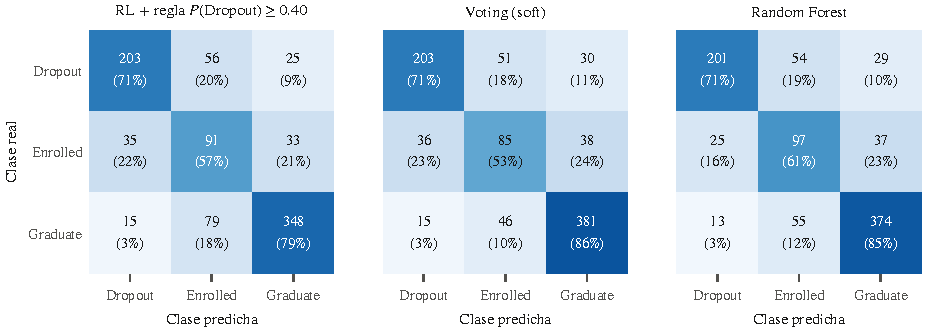
\includegraphics[width=\textwidth]{fig_confusion.pdf}
\caption{Matrices de confusión en Test (conteos y porcentaje por fila) de la RL con regla, Voting (soft) y Random Forest.}
\label{fig:conf}
\end{figure*}

\begin{table}[t]
\caption{Desempeño por clase en Test. D = Dropout, E = Enrolled, G = Graduate. F1 por clase, exhaustividad (Exh.) de E y desertores detectados (Det., de 284).}
\label{tab:clases}
\centering\scriptsize
\setlength{\tabcolsep}{3pt}
\begin{tabular}{@{}>{\raggedright\arraybackslash}p{2.55cm}ccccc@{}}
\toprule
Modelo & F1 D & F1 E & F1 G & Exh. E & Det. \\
\midrule
Regresión logística (RL) & 0.749 & 0.493 & 0.824 & 0.623 & 195 \\
RL + regla $P(\mathrm{Dropout})\geq0.40$ & 0.756 & 0.473 & 0.821 & 0.572 & 203 \\
SVM RBF & 0.761 & 0.451 & 0.858 & 0.403 & 208 \\
Random Forest & 0.769 & 0.532 & 0.848 & 0.610 & 201 \\
Voting (soft) & 0.755 & 0.499 & 0.855 & 0.535 & 203 \\
EBM & 0.747 & 0.517 & 0.826 & 0.667 & 195 \\
\bottomrule
\end{tabular}
\end{table}


\textbf{Variables más influyentes.} La Fig.~\ref{fig:imp} muestra la importancia por permutación (caída del \Fm{} en Test al permutar una variable) de Random Forest y de Voting (soft). Domina el número de UC aprobadas en el segundo semestre (\impRFASeg{} y \impVSASeg{}), seguido de la colegiatura al corriente (\impRFTF{} y \impVSTF) y de las UC aprobadas del primer semestre (\impRFAPri{} en Random Forest). Es coherente con el exploratorio (Fig.~\ref{fig:eda}) y con los trabajos previos sobre este conjunto \cite{praptomo2026}. Como se calculó en Test y después de seleccionar, la tomamos como descriptiva; la importancia por impureza (MDI) y la de permutación se parecen solo moderadamente ($\rho=\rhoMDI$).

\begin{figure}[t]
\centering
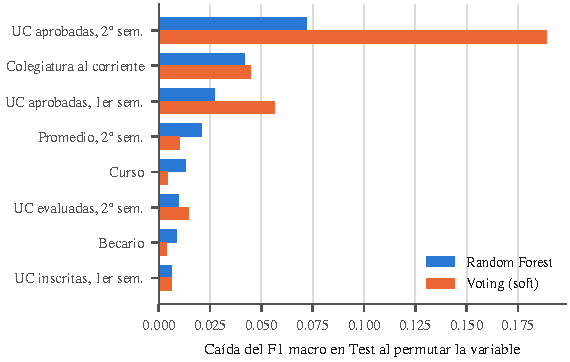
\includegraphics[width=\columnwidth]{fig_importancia.pdf}
\caption{Importancia por permutación en Test (caída del \Fm{}) de las ocho variables principales de Random Forest, y su valor para Voting (soft).}
\label{fig:imp}
\end{figure}

\subsection{Discusión}\label{sec:disc}
\textbf{¿Cuál es el mejor modelo?} Depende del criterio y no hay un ganador claro. Con \Fm{}, el criterio principal, Voting (soft) (\cvFVS) y Voting (hard) lideran en validación y Random Forest (\teFRF) en Test, pero las diferencias son pequeñas frente a la incertidumbre y, en validación cruzada repetida, ninguna sobrevive a la corrección por comparaciones múltiples. Con exactitud en Test, cuatro modelos superan a la RL con regla de forma significativa, pero no a la RL por defecto (\accLRD{}), y su AUC no se distingue del de la RL: lo que cambia entre modelos es sobre todo dónde se coloca el umbral entre \cE{} y las otras clases, no cuánto separan a los estudiantes. Si se prioriza simplicidad e interpretabilidad, la RL (\Fm{} de \teFLR{} en Test y \cvFLR{} en validación) queda a unos 0.02--0.03 de los mejores; si se prioriza detectar desertores, la RL con regla (\detLRR{} de 284) y las SVM (\detSVR{} para la RBF) son competitivas.

\textbf{Base frente a optimizado.} Optimizar sube la validación (\dcvMedia{} en promedio) pero no de forma confiable el Test (\dteMedia{}); parte de la ganancia en validación es optimismo de la búsqueda (hasta \optMax{}) y parte se explica por configuraciones base débiles (AdaBoost, SVM). En estos datos, partir de una configuración base razonable captura la mayor parte del rendimiento y la búsqueda aporta poco por encima de ella.

\textbf{Características de los datos.} La señal está concentrada en pocas variables del rendimiento académico, por lo que modelos de familias muy distintas alcanzan \Fm{} parecidos: el techo parece venir de la clase \cE, ambigua por construcción, y no de la capacidad del modelo. Un trabajo futuro con información más fina (asistencia, plataforma de aprendizaje) podría moverlo más que otro algoritmo.

\textbf{Comparabilidad.} Las cifras de la literatura solo son comparables cuando comparten partición, métrica y ausencia de fuga (Sec.~\ref{sec:sota}); en esos casos los resultados son equivalentes dentro del ruido.

\textbf{Limitaciones.} (i) Una sola partición con \Nte{} estudiantes: los intervalos miden unos $\pm0.03$ y no incorporan la variabilidad de la partición. (ii) Una sola institución y sin validación temporal: los indicadores macroeconómicos identifican cohortes y los modelos podrían aprender la cohorte. (iii) El predictor incluye el rendimiento de los dos primeros semestres: sirve como alerta tras el segundo semestre, no al ingreso. (iv) Los intervalos bootstrap pareados en Test no se corrigieron por multiplicidad (solo los McNemar, con Holm), McNemar no recoge la variabilidad del entrenamiento \cite{dietterich1998} y la importancia por permutación usó Test \emph{a posteriori}. (v) Con la validación cruzada de 5 folds para seleccionar y la repetida para inferir, la selección no es anidada; el optimismo observado es pequeño, pero no nulo. (vi) No se evaluó XGBoost, LightGBM ni CatBoost, usados por los trabajos citados; HistGradientBoosting es una variante cercana. (vii) Se trabajó sin remuestreo sintético, por lo que no se sabe cuánto cambiaría el resultado con SMOTE dentro de los folds.

\textbf{Trabajo futuro.} Validación anidada o con repetición de particiones; separación temporal por cohorte; calibración de probabilidades y umbrales por clase según el costo de cada error; modelos de alerta más temprana (inscripción y primer semestre), como en \cite{martins2023}; y explicaciones con SHAP, como en \cite{praptomo2026}.

%=====================================================================================================================
\section{Conclusiones}\label{sec:conc}
Con un protocolo sin fuga de información, una misma partición y los mismos folds, se compararon RL, SVM y diez familias de ensambles para clasificar a los estudiantes del conjunto UCI 697 en \cD, \cE{} y \cG. Los resultados responden al objetivo de la siguiente manera:
\begin{enumerate}
\item Los ensambles aportan mejoras \emph{modestas} sobre una RL bien configurada: en validación, \Fm{} de \cvFMinOpt{} a \cvFMaxOpt{} frente a \cvFLR{}; en Test, de \testFMin{} a \testFMax{} frente a \teFLR{}.
\item No se puede afirmar un modelo superior en el criterio principal. Voting (soft) lidera en validación (\cvFVS) y Random Forest en Test (\teFRF), pero en validación cruzada repetida ninguna diferencia frente a la RL es significativa tras el ajuste de Holm, y el orden de validación no predice el de Test (Spearman \rhoCVTest). En Test, \nMcnHolm{} modelos aciertan significativamente más estudiantes que la RL con regla (McNemar con Holm), pero su AUC es indistinguible y la RL por defecto los supera en exactitud: es compatible con un punto de operación distinto, no con mejor discriminación.
\item La optimización de hiperparámetros mejoró la validación (\dcvMedia{} en promedio) pero no de forma confiable el Test (\dteMedia{}).
\item El límite común es la clase \cE{} (F1 de 0.45 a 0.53), no la elección del algoritmo.
\item Las comparaciones con otros estudios son prudentes: solo dos comparten partición y métrica con este trabajo y, con ellos, la evidencia es de equivalencia dentro del ruido; las cifras más altas coinciden con protocolos distintos.
\end{enumerate}
La contribución principal es metodológica: un flujo reproducible que separa entrenamiento, selección y evaluación final, y que cuantifica la incertidumbre antes de declarar mejoras. El trabajo futuro más valioso es la validación temporal y la alerta más temprana.

%=====================================================================================================================
\balance
\bibliographystyle{IEEEtran}
\bibliography{refs}

\end{document}
